% DOCUMENT FORMAT ======================= -*- mode: LaTeX; coding: utf-8 -*- ===

%\documentclass[diploma]{report}
\documentclass[11pt,a4paper,english,greek,twoside]{report}

% PACKAGE SETTINGS =============================================================

\usepackage{fontspec}
\usepackage{amsmath}
\usepackage{amsfonts}
\usepackage{multirow}
\usepackage{array}
\usepackage{mdwlist}
\usepackage{subfig}
\usepackage{floatrow}
%\usepackage{float}
\usepackage{verbatim}
\usepackage{color}
\usepackage{graphicx}
\usepackage{xunicode}
\usepackage{xltxtra}
\usepackage{url}
%\usepackage{dsfont}
%\usepackage{microtype}
\usepackage{hyphenat}
\usepackage{multicol}
\usepackage{wrapfig}
\usepackage{lipsum}
\usepackage{listings}
\usepackage{paralist}
\usepackage{ulem}

% FONT SETTINGS ===============================================================

%\setromanfont[Mapping=tex-text]{CMU Serif}
%%\setromanfont[Mapping=tex-text]{CMU Sans Serif} % temporary change until printing
%%\setsansfont[Mapping=tex-text]{CMU Sans Serif}
%%\setmonofont[Mapping=tex-text]{CMU Typewriter Text}
%\setmainfont[Mapping=tex-text]{CMU Serif}
%%\setmainfont[Mapping=tex-text]{CMU Sans Serif}  % temporary change until printing

%\setromanfont[Mapping=tex-text,ExternalLocation=fonts/]{cmunrm.otf}
%\setsansfont[Mapping=tex-text,ExternalLocation=fonts/]{cmunss.otf}
%\setmonofont[Mapping=tex-text,ExternalLocation=fonts/]{cmuntt.otf}
%\setmainfont[Mapping=tex-text, ExternalLocation=fonts/]{cmunss.otf}

\defaultfontfeatures{Mapping=tex-text}
%\setromanfont{Linux Libertine O}
\setromanfont{Times New Roman}

% CUSTOM COLORS ===============================================================

\definecolor{gray}{rgb}{0.5,0.5,0.5}
\definecolor{darkgreen}{rgb}{0.0,0.5,0.0}
\definecolor{mygreen}{rgb}{0,0.6,0}
\definecolor{mygray}{rgb}{0.5,0.5,0.5}
\definecolor{mymauve}{rgb}{0.58,0,0.82}
\definecolor{myorange}{RGB}{246,177,50}

% CUSTOM COMMANDS =============================================================

\newcommand\fixme{\textrm{\textbf{\textcolor{red}{FIXME: }}}}
\newcommand\todo{\textrm{\textbf{\textcolor{myorange}{TODO: }}}}
\newcommand\mytilde{\raise.17ex\hbox{$\scriptstyle\sim$}}
\newcommand\okeanos{\textbf{\raise.17ex\hbox{$\scriptstyle\sim$}okeanos }}


% Layout macros
\newcommand\spa[1]{\; #1 \;}

% Font macros
\newcommand\resfont[1]{\ensuremath{\mathtt{#1}}}

% Mathematical macros
\newcommand\setmap[3]{#1\{#2 \mapsto #3\}}
\newcommand\getmap[3]{(#2 \mapsto #3) \in #1}
\newcommand\tuple[2]{\ensuremath{\langle#1, #2\rangle}}
\newcommand\mfrac[2]{\ensuremath{\dfrac{#1}{#2}}}
\newcommand\nequiv[2]{\ensuremath{#1 \not\equiv #2}}

% Core Ruby Operational Semantics letter bindings
\newcommand\mem{\mu}

% Core Ruby Operational Semantics low level macros
\newcommand\state[2]{(#1, #2)}
\newcommand\transition[1]{\ensuremath{\overset{#1, c*}{\rightarrow}}}
\newcommand\range[2]{#1, ..., #2}
\newcommand\midrange[5]{\range{#1}{#2}, #3, \range{#4}{#5}}

% Core Ruby Operational Semantics high level macros
\newcommand\operation[5]{\ensuremath{\state{#1}{#2} \transition{#3} \state{#4}{#5}}}
\newcommand\propagation[2]{\operation{#1}{\mem}{#2}{#1'}{\mem'}}

% Core Ruby specific Operational Semantics macros
\newcommand\semicolon[2]{#1; \; #2}
\newcommand\assign[2]{#1 = #2}
\newcommand\mcall[3]{#1.\texttt{#2}(#3)}
\newcommand\ifte[3]{\resfont{if} \; #1 \; \resfont{then} \; #2 \; \resfont{else} \; #3}
\newcommand\newclass[2]{#1.\resfont{new}(#2)}
\newcommand\methoddef[3]{\resfont{def} \; #1(#2) = #3}
\newcommand\classdef[2]{\resfont{class} \; #1 = #2}
\newcommand\with[3]{with \; \tuple{#1}{#2} \; do \; #3}

% Success Typing macros
\newcommand\ssub{\sqsubseteq\_S}

% Core Ruby Success Typing letter bindings
\newcommand\classlist{\Delta}
\newcommand\envir{\Gamma}
\newcommand\fields{\Phi}
\newcommand\currclass{l}

% Core Ruby Success Typing inferencing macros
\newcommand\stinfer[5]{\classlist; \; #1; \; \fields \; \underset{\currclass}{\vdash} \; #2: #3 \; \& \; #4; \; #5}


%%%%%%%%%%%%%%%%%%%%%%%%%%% CACHED STUFF %%%%%%%%%%%%%%%%%%%%%%%%%%%

\newcommand\xcache{\texttt{xcache} }

%%%%%%%%%%%%%%%%%%%%%%%%%%% HASKELL STUFF %%%%%%%%%%%%%%%%%%%%%%%%%%%

%\newcommand\typerep[1]{\ensuremath{#1}}
\newcommand\typerep[1]{\lstinline[basicstyle=\normalsize\ttfamily,keywords={}]|#1|}
\newcommand\typefootrep[1]{\textbf{\lstinline[basicstyle=\footnotesize\ttfamily,keywords={}]|#1|}}
% \newcommand\ttyperep[1]{\typerep{#1}}
% \newcommand\mtyperep[1]{\mbox{\typerep{#1}}}

% Arrow types
\newcommand\typeto[2]{\typerep{#1} \typerep{->} \typerep{#2}}
\newcommand\typetotwo[3]{\ensuremath{\typerep{#1} \typerep{->}
                                     \typerep{#2} \typerep{->}
                                     \typerep{#3}}}

\newcommand\tyconapone[2]{\ensuremath{\mbox{\typerep{#1}} \:\: \mbox{#2}}}
\newcommand\tyconaponeC[2]{\ensuremath{\mbox{\typerep{#1}} \:\: \mbox{\typerep{#2}}}}
% \newcommand\tyconapone[2]{\typerep{#1} $\:$ \typerep{#2}}

\newcommand\tyconaptwo[3]{\ensuremath{\mbox{\typerep{#1}} \:\: \mbox{#2} \:\: \mbox{#3}}}


% FIGURE SETUP ===============================================================

\newcommand\diagram[2]{
	\begin{figure}[h!]
		\centering
		\includegraphics[width=\textwidth,height=\textheight,keepaspectratio]
		{diagrams/#2}
		\caption{#1}
		\label{fig:#2}
	\end{figure}
}

\newcommand\diagramstrict[2]{
	\begin{figure}[H]
		\centering
		\includegraphics[keepaspectratio]
		{diagrams/#2}
		\caption{#1}
		\label{fig:#2}
	\end{figure}
}


% SPELLING =====================================================================

% CODE HIGHLIGHTING ============================================================

% Define common settings for code listings

\lstset{
	backgroundcolor=\color{white},
	basicstyle=\small\ttfamily,		% style for code
	breakatwhitespace=false,        % sets if automatic breaks should only
									% happen at whitespace
	breaklines=true,                % sets automatic line breaking
	captionpos=b,                   % sets the caption-position to bottom
	commentstyle=\color{mygreen},   % style for comments
	escapeinside={\%*}{*)},         % if you want to add LaTeX within your code
	frame=single,                   % adds a frame around the code
	keepspaces=true,                % keeps spaces in text, useful for 
	%keywordstyle=\color{blue}\bfseries,
					% keyword style
	numbers=left,
	numbersep=5pt,                  % how far the line-numbers are from the 
					% code
	numberstyle=\tiny\color{mygray},% style for line-numbers
	rulecolor=\color{black},
	stepnumber=1,                   % the step between two line-numbers. If 
					% it's 1, each line will be numbered
	stringstyle=\color{mymauve},    % style for strings
	tabsize=2,                      % sets default tabsize to 2 spaces
}

% Define specific rules for each language

\lstdefinestyle{c}
{
	language=C,
	tabsize=4
}

\lstdefinestyle{haskell}
{
	language=Haskell
}

\lstdefinestyle{ruby}
{
	language=Ruby
}

\lstdefinestyle{erlang}
{
	language=Erlang.
	captionpos=
}

\lstdefinestyle{plain}
{
	stepnumber=0
}

% Create new commands for simpler usage

\newcommand\ccode[2]{
	\lstinputlisting[float=h!, style=c, caption={#1}, label=lst:#2]{src/#2}
}

\newcommand\haskellcode[3]{
	\lstinputlisting[style=haskell, caption={#1}, label=lst:#2]{src/#3}
}

\newcommand\rubycode[2]{
	\lstinputlisting[style=ruby, caption={#1}, label=lst:#1]{src/#2}
}

\newcommand\erlangcode[2]{
	\lstinputlisting[style=erlang, caption={#1}, label=lst:#1]{src/#1}
}

\newcommand\plaintext[2]{
	\lstinputlisting[float=h!, style=plain, caption={#1}, 
	label=lst:#2]{src/#2}
}

% CHANGE MATH FONT ============================================================

% HYPERREF MUST BE LAST =======================================================

\usepackage[xetex,colorlinks=true,linkcolor=blue,citecolor=darkgreen]{hyperref}

% DOCUMENT INFORMATION =========================================================

\title{Σχεδίαση και Υλοποίηση Μηχανισμού Κρυφής Μνήμης για Κατανεμημένο Σύστημα 
	Αποθήκευσης σε Περιβάλλον Υπολογιστικού Νέφους} 

% ===============> FIXME
\author{Αλέξιος Πυργιώτης}
\authoren{Alex Pyrgiotis}
\datedefense{8}{1}{2014}
\supervisor{Νεκτάριος Κοζύρης}
\supervisorpos{Καθηγητής Ε.Μ.Π.}
\committeeone{Νεκτάριος Κοζύρης}
\committeeonepos{Καθηγητής Ε.Μ.Π.}
\committeetwo{Νικόλαος Παπασπύρου}
\committeetwopos{Αναπ. Καθηγητής Ε.Μ.Π.}
\committeethree{Δημήτριος Φωτάκης}
\committeethreepos{Επίκ. Καθηγητής Ε.Μ.Π.}

\hypersetup{
	pdftitle={},
	pdfauthor={Alex Pyrgiotis},
	pdfsubject={},
	pdfkeywords={}
}


% MAIN DOCUMENT ================================================================

\begin{document}

\frontmatter
\maketitle

\def\templen{\parindent}
\setlength{\parindent}{0pt}
\setlength{\parskip}{1.5ex plus 0.5ex minus 0.2ex}
\begin{acknowledgements}

Θα ήθελα να ευχαριστήσω τον επιβλέποντα καθηγητή κ. Νικόλαο Χατζηαργυρίου για την ευκαιρία που μου έδωσε να εκπονήσω τη παρούσα διπλωματική και την υποστήριξή του σε όλη την πορεία της.

Επίσης, θα ήθελα να ευχαριστήσω  τους καθηγητές κ. Σταύρο Παπαθανασίου και κ. Παύλο Γεωργιλάκη για την τιμή που μου έκαναν να συμμετάσχουν στην επιτροπή εξέτασης της διπλωματικής.

Eυχαριστώ ιδιαίτερα τον υποψήφιο διδάκτορα Γιώργη Μεσσήνη για την καθοδήγηση, στήριξη και καθοριστική βοήθεια που μου παρείχε.

Τέλος, θα ήθελα να ευχαριστήσω την οικογένειά μου και τους φίλους μου που παρέχουν πάντοτε ένα χέρι βοήθειας σε ό,τι χρειαστώ.

\end{acknowledgements}


\begin{abstract}
Οι εταιρίες παροχής ηλεκτρισμού αντιμετωπίζουν το ολοένα και αυξανόμενο πρόβλημα της διείσδυσης μη τεχνικών απωλειών στις καταναλώσεις των πελατών τους. Το γεγονός αυτό πλήττει σημαντικά τις εταιρίες, μειώνοντας το εισόδημά τους και θέτει σε κίνδυνο τους ανειδίκευτους καταναλωτές που επεμβαίνουν στις υποδομές του παρόχου. Η προσέγγιση αυτού του προβλήματος έγινε με προσομοίωση ρευματοκλοπών σε ετήσιες χρονοσειρές καταναλωτών και δοκιμάστηκαν πληθώρα αλγορίθμων επιβλεπόμενης, μη επιβλεπόμενης και ημι-επιβλεπόμενης μηχανικής μάθησης για την ανίχνευση των καταναλωτών με διείσδυση μη τεχνικών απωλειών. Τα αποτελέσματα αναδεικνύουν τις δυνατότητες των συστημάτων μη επιβλεπόμενης και ημι-επιβλεπόμενης μάθησης σε σχέση με τη δεδομένη επιτυχία των αλγορίθμων επιβλεπόμενης μάθησης. Τα συστήματα που δημιουργήθηκαν έχουν ικανοποιητική απόδοση που δεν αποκλίνει σημαντικά από τους αλγορίθμους αναφοράς της επιβλεπόμενης μάθησης. Καθίσταται λοιπόν σαφές πως η ανίχνευση μη τεχνικών απωλειών είναι εφικτή με συστήματα μηχανικής μάθησης.

\begin{keywords}
  Μη τεχνικές απώλειες, Ρευματοκλοπές, Χρονοσειρές, Μηχανική μάθηση, Επιβλεπόμενοι αλγόριθμοι, Μη επιβλεπόμενοι αλγόριθμοι, Ημι-επιβλεπόμενοι αλγόριθμοι.
 
\end{keywords}

\end{abstract}



\begin{abstracteng}
\tl{Power companies face the problem of increasing intrusion of non-technical losses on consumptions of their clients. That fact hurts significantly power companies by reducing their economical growth and sets on danger unskilled consumers who intervene with the power infastracture. This problem was approached by simulating frauds on yearly timeseries and by testing  many different algorithms of supervised, unsupervised and semi-supervised  machine learning in order to detect consumers with non-technical loss intrusion. The results show the potencial of the unsupervised and semi-supervised learning in relation with the given success of supervised algorithms. The created systems have satisfactory performance which does not diverge significantly from the reference algorithms of supervised learning. Concluding the detection of non-technical losses is achievable with machine learning systems.}
\begin{keywordseng}
  \tl{Non-technical losses, power fraud, Timeseries, Machine learning, Supervised algorithms, Unsupervised algorithms, Semi-supervised algorithms.}
\end{keywordseng}

\end{abstracteng}


\setlength{\parindent}{\templen}
\setlength{\parskip}{0pt}
\tableofcontents
\listoffigures
\listoftables
\renewcommand{\lstlistlistingname}{List of Listings}
\lstlistoflistings % changed the title above

\mainmatter
% moved these two commands here so that they don't influence the toc
\setlength{\parindent}{0pt}
\setlength{\parskip}{1.5ex plus 0.5ex minus 0.2ex}

\renewcommand\floatpagefraction{.7}

\chapter{��������}
� ���������� ����� �������� ���� ���������� ��������� �����
�����������. ������, � ����������� ���������� ��� ����������� ���
�����, ����� ���������������� ���� ��� �������-������ ��� ���
����� ��������� ��� ��� ���������. ��� �� ����������� ������ �
��������� ���������� ��� �� ����� ��� ������ � ��������� ��� �
����������� ���, � ���������� ����� ����������� ��� �������������
����.

� �������������� �����, ����� ��� ������� ��� ��������� �����,
���� ���� ����� ������� ���� �������� ����� ���� ���������� ���
�����������, �������������� �� ���������� ������ ���������� ���
�������� \cite{Berners-Lee01}. ��� ������������ ����� ��
���������� ��������� ��������� �� ������ ���� ����� �����������,
����� ��� ��� ��������������� ���������� ��� �����������,
��������������� �������� ��� ��� ����������� ��� �����������
$``$������������$"$. � �������� ����� ��� ��������, ��� ������ ���
��� ��������� ��� ����� ����������� ��������� �� ����������
��������� �� ����� ��� ����� ��� ��� �������� ����������� ���
������������ ��� ������� ��������� ��� ��������� ����� ���
�������� ��� ��� ���� ��� ������ ��� �����������.

��� ��� �� ��� ������ ������ ��� ��� �������� ��� ��������������
����� ����� �� �� ������� �� ����������� �� ������������ ��������
 ������ ���������. �� ��� ������� ���������� ����
����� � �������������� ����� ���������� ��� �������� ��� ��������
������� ���������� ��������� ���� ����� �� ��������� ��������
������ \en{(Peer-to-Peer systems)}.

��� ������� �������� ������ ����������� ��� ��� ������ ���������
������������� ������, �� ������ ������������� �� ����� ���
��������� ���������. �� ��������� �������� ������ ���
���������������� ������ ������ ������ ��� ��� ��������� �������
��������, ����� ���� ������ ����������� ����������� ���������. �
��������� ����������� ��� ����������� ��� ���� ������� �� �����
������ �������� \en{(keyword-based search)}.

� ������ ��� ��� ����������� �����������, �� ��������� �� ���
�������� ��� �������������� �����, ������� ��� ��������� ��������
������ ��� ����� ��������� �� ������� \en{(schema-based
peer-to-peer systems)}. ��� ��������� ���� ���� ������
������������ ��� ����� �� ���� �� ����� ��������� �� ������
��������� ��������. �� ����������� ��� �������������� ����� ������
�� ���������� ��������� ��� ��������� ���� �������� ��� ��
�����������.

�� ������� \en{RDF} ����� ��� ������ �������� �������������
�������������. �� ��� \en{RDF} ������ ��������� �������� ���
����������� ��� ����� ���� �������, ����������, ����������� �.�.�.
��� �������� ��� �������� \en{RDF} ����� �� \en{RDF Schema} ��
����� ������� ����������� ���������� �������� ������������ ���
����� ����� ��� ��� ������� ������ ����. �� \en{RDF Schema}
��������� �� ������� ��� ��������� ������� ������� ��� �� ���� ���
������������������ ����������. � ������ ������� ����� ��� ���
������� \en{RDF} �� ��������� ��������� ���������� ��� ���
�������.

��������������� ������ ��� ����������� ��� �������������� �����
�������� �� �������������� ��������� �������� ������ �� ��������
������������������ �� ����� �� ������������ ������ ���� ����������
�� ����� ��� �� ����� �� ���������� ���������� ��������� ���
����������� ��� ����� ��� ���������� �� ������ �������.


\section{����������� ��� ������������}
�� ������ ������ ��� ��������� ��� �� ��������� �������� ������
��� ����� ��������� �� �������, ����� ��� �� ������� �� ������ ��
��������� ��� �� ������������ ��������, ����������� ��� ���������
����. ��� ������������ ����� �������� ���� ������������:
\begin{enumerate}
\item � ����� ���������� ������� �� ������� ��� �������� ����� ��
����� �� ������������� ���� �� ������ \cite{KokkinidisC04}. ��
��������� ������������� ��� ������������ �� ���� �� ���� �����.
��� ������ ���� �� ���� ���� ��� ������������ �� ����������� ����,
���� ��� ���������� �� ������ ������ ���� ����������. ���� �� ���
������� ���������� ���� ����� � ���������� ����� ���������� ���
��� �������� ������� ��� �� ��������� ��� ����� ������ ��������.
\item � ������� ���������� ����� ��� ��������� �� ���� ����� �� �������� ����� ����� �����.
�� ��������� ������������� �� ���� ��� ����� ��� ������������ ��
���� ���� �������, ���� ���� ����������� ��������������� ���������
\en{(query reformulation)}. � ���������� ���� ������� ��� ������
������� ������������� \en{(mapping rules)} \cite{Piazza}. ����, ��
��� ������� �������� ������ �� ������ ������� �� �������� ��� ��
�������� ��� ������ �������. ��� ����� ������ �������� �� ���
�������� �� �������� ��� ������ ������ ��� ������ ������ ��
�������� ������� �������������. ������, �� ������� �����
���������� ������������ ��� ����� ������� � ��������� ����.
\end{enumerate}

����������� ��� ������������ ����� � �������� ���� ����������
�������� ������ ��������� �� ������� �� ����� (�) �� ��������� ���
������� �������� ���� ����� ��� �������� ��� (�) �� ����� ���
���������� ��������������� ��������� ����� ��� ������ ����������
������� ������������� ������ ��������. �� ������� ������ ���������
������� ��� ��� ������� ��� ������������ ��������, ��� �������
��������� ��� ����� �� ���������� ��������� ���������������
���������. ������������ ������� �� ������� \en{RDFS} ��� ���������
���������-����� \en{(views)} ���� ������� �������� (��������
�����).

��� ���������� ��������� ��� ���������� ����� �� ���� � ���������
�������������� ��������� ������ ��� ���������. ���� ��������� ��
���������� �� ���� �� ������� �������� ������ �� ��� ���� ���
\en{RDF} ����� ������� �� �� ����� �� �������� ��� ������������
��� ��� ���������� �� �������� �� ���������� ������� �������� ���
������ �������. �' ��� ������ ������� �� ��������� �� �����������
�� ������ ����� ��� ����������� ��������� ��� ���������� � ���
��������.

\section{�������� ��� �����}
� ������� ���� ����� ���������� �� ���� ��������: ��� �������� 2
������� �� ��������� �������� ��� ������� ����������� ���
����������� �� �� ����������� ����. ������ ������������� �� ������
�������� ������, ��� �������� �� ������� \en{RDF} ��� �����
������� ��� ������ ��� ������� ��������� ��� \en{RDF}. ���
�������� 3 ������ ������������� �� �������� �� �� ���� ��������
��� ��� �������� ������� � ������ ��� ������������� ��������. ���
�������� 4 ������������� � ������� ��� � �������� ��� ����������,
������ � ��������� ��� ������������� ��� ��� ��������� ���. �
��������� ��� ���������� ��� ����������, �� ������� ��� �������
���������� ����� ��� ������������ ������� �� ��� ���������� ��� ��
���������������� �������� ��� ���������������� ������� ���
�������� 5. ��� �������� 6 ������������� � ������� �����
����������� ��� ���������� �� ���� ��� ������������ �������
������. ����� ��� �������� 7 ������� � ���������� ����� ���
������������ ��������, ����� ��� ����������� ����������.

\chapter{Necessary theoretical background}\label{ch:theory}

In this chapter, we will explain the main concepts and mechanisms that are used 
by Archipelago as well as our implementation. The concepts that will be 
discussed are basic as far as Operating Systems are concerned and should pose 
no comprehension difficulties to a reader with elementary background on the 
subject.

More specifically, Section \ref{sec:multi-theory} discusses what is 
multithreading and lists its advantages and disadvantages. Section 
\ref{sec:ipc-theory} introduces the Interprocess Communication mechanisms that 
are employed by Linux and concentrates on the ones that are used in Archipelago 
and our implementation. Finally, Section \ref{sec:conc-theory} explains the 
various concurrency control methods that exist to synchronize threads or 
processes.

\section{Multithreading}\label{sec:multi-theory}


Mutlithreading is a programming concept that has been the subject of research 
long before the emerge of SMP systems\footnote{
	Symmetric multiprocessing systems, commonly systems with multiple 
	processors}. More specifically, temporal multithreading has been introduced 
in the 1950s whereas simultaneous multithreading (SMT), which is the current 
invocation of multithreading programming, was first researched by IBM in 
1968\cite{mt}.

The difference between these two types is the number of threads that can run 
simultaneously on the system. For simultaneous multithreading, there are 
commonly more than one threads that can run in parallel, whereas for temporal 
multithreading, there is only one. This means that the running thread must be 
descheduled to let the other threads run. Temporal multithreading was an old 
concept that predates SMP systems and this limitation mirrors the limitations 
of the hardware of that era.

Before threads, programs could utilize the concurrency of SMP systems using 
forked processes that would communicate with each other. The introduction of 
threads did not render this practice obsolete, but instead provided an 
alternative technique to speed up applications.

Threads and process have some fundamental differences, which are shown in the 
following list:

\begin{itemize}
	\item Threads are always parts of a process, whereas processes are 
		independent from each other and may only have a parent-child connection 
		between them.
	\item Forked processes have their own address space and resources, which 
		are inherited by the parent process with CoW semantics.  Multiple 
		threads, on the other hand, usually share the same memory and resources 
		with the other threads in the same process.
\end{itemize}

From the above differences, we can see that there are no clear advantages of a 
multithreaded approach over a multiprocess one. To better demonstrate our 
point, we will present the advantages and disadvantages of multithreading 
programming in the following lists:

The advantages are:

\begin{itemize}
	\item Context switching is generally faster between threads, mostly due 
		to the fact that the TLB
		\footnote{Translation Lookaside Buffer, a hardware cache that speeds up 
			the translation of virtual addresses to physical RAΜ pages.}
		cache does not need to be flushed. The TLB cache misses are 
		expensive and are avoided as much as possible\cite{tlb}.
	\item Sharing data between threads is easier, due to the fact that they 
		use the same memory by default.
\end{itemize}

Whereas the disadvantages are:

\begin{itemize}
	\item Processes are more isolated than threads, which means they are 
		guarded against two things:
		\begin{inparaenum}[i)]
		\item thread-unsafe functions and
		\item data corruptions, which if they happen to one thread they 
			bring the whole process to a halt.
		\end{inparaenum}
\end{itemize}

Regardless of the chosen method, at some point the programmer will have face 
two of the biggest challenges of multithreading/multiprocess programming;
interprocess communication, which is discussed in Section \ref{sec:ipc-theory}, 
and concurrency control, which is discussed in Section \ref{sec:conc-theory}.

\section{Interprocess Communication - IPC}\label{sec:ipc-theory}

Interprocess Communication is a concept that predates the SMP systems that we 
all use nowadays. It is a set of methods that an OS uses to allow processes and 
threads to communicate with each other. Archipelago for example, uses various 
IPC methods to synchronize its different components.

The full list of Linux's IPC methods is presented below:

\begin{itemize}
	\item \textit{Signals,} which are sent to a process to notify it that 
		an event has occurred.
	\item \textit{Pipes,} which are a one-way channel that transfers 
		information from one process to another.
	\item \textit{Sockets,} which are bidirectional channels that can 
		transfer information between two or more processes either 
		locally or remotely through the network.
	\item \textit{Message queues,} which is an asynchronous communication 
		protocol that is used to exchange data packets between 
		processes.
	\item \textit{Semaphores,} which are abstract data types that are used 
		mainly for controlling accesses on a same resource.
	\item \textit{Shared memory,} which is a memory space that can be 
		accessed and edited by more than one process.
\end{itemize}

We will concentrate on the following IPC methods:
\begin{inparaenum}[i)]
\item signals,
\item sockets and
\item shared memory,
\end{inparaenum}
since these are the methods that Archipelago and our implementation use.

\subsection{Signals}

Signals are notifications that are sent to processes and can be considered as 
software interrupts. The signal's purpose is to interrupt the execution of a
process and inform it that an event has occurred.

Given that there more than one events and exceptions that can occur in a 
system, there are also various signals that match to each one of these
events. For more information about the signals that Linux supports as well as 
the conditions on which they are raised, the reader is prompted to consult the 
man pages for signal(7) or read the POSIX.1-1990, SUSv2 and POSIX.1-2001 
standards.
  
Moreover, the above standards dictate the standard behavior of a process when a 
signal is received. The standard actions that a process can take, fall roughly 
in the following categories:

\begin{itemize}
	\item ignore the signal,
	\item pause its execution,
	\item resume its execution or
	\item stop its execution and/or dump its core
\end{itemize}

Finally, a process is not limited to this set of actions. It can instead do one 
of the following things for each signal, with the exception of SIGKILL and 
SIGSTOP signals:

\begin{itemize}
	\item ignore the signal
	\item block the signal, which is part of the Archipelago IPC and its 
		usage is described in Section ?
	\item install a custom signal handler function, which essentially 
		passes the signal handling task to the process.
\end{itemize}

\subsection{Sockets}

Sockets are a bidirectional means of sending data between processes.  The 
processes can be in the same host but most commonly, they are in remote hosts 
and the data are sent over the network. Furthermore, from all the IPC methods 
that we have described above, sockets are the only method that enables remote 
communication. 

There are many socket implementations for different purposes, which are divided 
in several communication domains, most of which are rather obscure. The three 
communication domains, however, that are supported by most UNIX and UNIX-like 
operating systems are:

\begin{itemize}
	\item \textit{IPv4} domain, which allows communication between 
		processes over the Internet Protocol version 4 network.
	\item \textit{IPv6} domain, which allows communication between 
		processes over the Internet Protocol version 6 network.
	\item \textit{UNIX} domain, which allows communication between 
		processes in the same host
\end{itemize}

The above three communication domains are further divided in two types, based 
on the transport layer protocol that they use.

\begin{itemize}
	\item \textit{Stream sockets}, which use the Transmission Control 
		Protocol (TCP) or Stream Control Transmission Protocol (SCTP),
	\item \textit{Datagram sockets}, which use the User Datagram Protocol 
		(UDP),
\end{itemize}

The TCP/UDP protocols are only one layer out of the four layers of the TCP/IP 
protocol stack that the RFC 1122\cite{1122} defines, and we will explain them 
in detail in the following sections.  Although a thorough explanation of the 
TCP/IP protocol stack is out of the scope of this thesis and is not needed to 
understand the following sections, we will provide a brief explanation of it 
for the sake of completeness.  

The TCP/IP protocol stack is the basis for the World Wide Web and the most used 
form of networking. It specifies all the stages of the data processing that 
need to happen in various levels and entities, such as operating systems, 
network cards, routers etc. in order to connect two machines over the network.  
For this reason, the data that are sent are encapsulated in layers, which can 
be seen in Figure \ref{fig:data-encapsulation.pdf}.

\diagram{Data encapsulation for a UDP packet}{data-encapsulation.pdf}

We now continue with an presentation of TCP and UDP protocols.

\subsubsection{TCP}

The Transmission Control Protocol is connection-oriented, i.e. it provides 
unique connection between two sockets, and has the following key features:

\begin{description}
	\item[Reliability] The data will arrive to the receiver as a whole, or 
		they will not arrive at all. In the latter case, the receiver 
		may receive sparious packets but it will not acknowledge them 
		until it has received all of them.
	\item[Ordered transfer] The data will arrive in the same order that 
		they were sent.
	\item[Error-checking] The data are checksummed to allow the receiving 
		end to check if there was any data corruption.
	\item[Rate-limiting] When the receiver accepts packets with slower rate 
		than the sender, the sender will adjust its rate to ensure 
		packet delivery and less congestion.
	\item[Byte-stream] The data that are sent do not have a boundary.
\end{description}

\subsubsection{UDP}

The User Datagram Protocol on the other hand is a much simpler protocol. It is 
used to send \textit{datagrams}, which are basically extended IP packets with 
some extra features. The UDP protocol has the following differences from 
TCP:

\begin{itemize}
	\item It is connectionless, meaning that the socket can receive 
		requests from anyone.
	\item It provides no guarantees about the delivery of the messages.  
	\item The messages can arrive in other order than the one they were 
		sent.
	\item There is no rate-limiting, meaning that the congestion control 
		must be handled in the application level.
	\item It cannot send streaming data since datagrams are bounded.
\end{itemize}

The UDP protocol is often preferred over TCP by applications that value speed 
over data loss (e.g. video streaming applications) due to its low overhead.

\subsection{Shared memory}

When two or more processes share the same memory segment, they can exchange 
data by placing it in a region of the segment. The data then becomes instantly 
visible to the other processes too, since their page-table entries for this 
segment point to the same physical RAM pages.

A popular way of mapping shared memory to a process's address space, which is 
also used in Archipelago, is with POSIX \texttt{mmap()}. There are two mapping 
types of mapping:

\begin{itemize}
	\item \textit{Private mapping}, in which case the mapping contents will 
		not be visible to other processes that have mapped the same 
		file and
	\item \textit{Shared mapping}, in which case the mapping contents will 
		be visible to all processes that map this file and changes to 
		the mapping will be propagated to the shared memory.
\end{itemize}

Finally, an issue with mappings is that the start of the shared memory is not 
always mapped in the same virtual address for all processes. For this reason, 
when processes want to share data, they should not pass direct pointers to 
them, but relative pointers (i.e. offsets) from the start of the segment, which 
are common for all processes and can be translated to the correct direct 
pointers.

\section{Concurrency control\label{sec:conc-theory}}

Concurrency control is the set of methods that a program uses to ensure that 
concurrent accesses to the same data will leave them in a consistent state.

There are several techniques that are used for concurrency control and are 
listed below:

\begin{itemize}
	\item \textit{Spinlocks}, which are locks that protect a critical segment.  
		Typically, a thread acquires a lock at the start of the critical 
		segment and releases it at the end of it. Threads that are waiting for 
		the lock essentially "spin", i.e. they busy-loop until the lock is 
		released.
	\item \textit{Mutexes}, which are locks that protect a critical segment in 
		the same fashion as spinlocks. Their difference from spinlocks, however 
		is that if a thread cannot get the lock, it will block instead of 
		busy-loop.
	\item \textit{Semaphores}, which are also an IPC method. In concurrency 
		control context, they are abstract data types that restrict the 
		number of simultaneous accesses to a resource or a critical 
		segment.  When the number of times is one (1), they essentially 
		degenerate to mutexes, with the main difference that they have 
		no concept of an owner.
	\item \textit{Atomic operations}, which are hardware-assisted 
		operations whose purpose is to atomically update a value as 
		fast as possible. The atomicity is usually achieved with 
		implicit hardware locks on the bus or cache-line.  Atomic 
		operations come in many flavors such as "add-and-fetch", 
		"compare-and-swap" etc.
\end{itemize}

Concurrency control - and locking in particular - have three important caveats 
that the programmer needs to know before he/she decides on the techniques that 
will be used:

\begin{description}
	\item[Lock overhead] \hfill \\
		Lock overhead is the overhead that the locking mechanism 
		introduces.  For example, semaphores are a mechanism with big 
		overhead, since they must be read and written to using system 
		calls. If the critical segment they protect is simply the 
		update of a variable, then the programmer is probably better 
		off using a spinlock or atomic operations.
	\item[Lock contention] \hfill \\
		Lock contention can be considered as the overhead of the 
		coarseness of the lock. There is contention for a lock when it 
		is requested by many threads, to the point that the waiting 
		time is longer than the execution time.
		This has a big performance impact to the implementation, since 
		threads may consume their scheduled time spinning until they 
		acquire a lock, or sleeping while they could do something more 
		useful.
		The solution to this problem is commonly to redesign the 
		locking scheme in order to break such locks into smaller ones.
	\item[Deadlocks] \hfill \\
		Deadlock is a situation in a multi-lock scenario where each 
		process in a group of processes needs to acquire a lock which 
		is held by another process in the same group. Since no process 
		can continue, the operation of the group is essentially 
		stalled.

		\diagramstrict{Deadlock example}{deadlock.pdf}

		As a rule of thumb, the circular dependency of the locks can 
		break if the locks are acquired in a predefined order. This 
		however is only possible in less complex scenarios and in 
		general, a more well-thought design is required.
\end{description}

\chapter{Archipelago}\label{ch:archip}

This chapter presents Archipelago, a distributed storage layer that is part of 
the Synnefo cloud software. More specifically, Section 
\ref{sec:overview-archip} introduces Archipelago and its basic features.  
Section \ref{sec:arch-archip} shows the architecture of Archipelago and 
explains the components that it consists of. Section \ref{sec:req-archip} 
illustrates how Archipelago handles the I/O request flow up to the storage 
backend and finally, Section \ref{sec:rados-archip} shows an important 
Archipelago storage backend, the RADOS object storage.

\section{Overview}\label{sec:overview-archip}

Archipelago is a distributed storage layer that is part of the Synnefo cloud 
software. It is responsible for creating Copy-on-Write, snapshottable volumes 
for VMs.  Archipelago can be considered as a storage layer (see Figure 
\ref{fig:archipelago_overview_a.pdf}) that is positioned between the VM's block 
device, and the underlying storage. Also, we can see that it is distributed in 
nature since it can run in an arbitrary number of nodes and most importantly 
with zero communication overhead between them.

\diagram{Archipelago overview}{archipelago_overview_a.pdf}

Archipelago has the following objectives:

\begin{itemize}
	\item Thinly provision volumes to VMs with zero data movement.
	\item Snapshot VM volumes and use them as system images with, again, zero 
		data movement.
	\item Allow VM migrations between Archipelago nodes with no restrictions.
	\item Be agnostic to the actual storage backend used.
\end{itemize}

\section{Architecture}\label{sec:arch-archip}

Archipelago has a modular architecture, which allows it to categorize its 
operations and assign them to distinct components. The IPC between these 
components, which are called \textbf{peers} in the Archipelago dialect, is 
facilitated by XSEG.

XSEG can be considered as the kernel of Archipelago and is a custom mechanism 
that:
\begin{inparaenum}[i)]
\item defines a common communication protocol for all peers, regardless of 
	their type (userspace/kernelspace, singlethreaded/multithreaded) and
\item builds a shared memory segment, where peers can share data using 
	zero-copy techniques.
\end{inparaenum}
The above are provided to the peers by the \texttt{libxseg} library.

In Figure \ref{fig:new_sxima_numbered.pdf}, we present the architecture of 
Archipelago.  Moreover, we show the Archipelago peers, the communication 
channels between them and we briefly explain the operations that they are 
responsible for.

\diagram{Archipelago components}{new_sxima_numbered.pdf}

\begin{description}
	\item[XSEG Block Device (xsegbd)] \hfill \\
		xsegbd is a kernel module that exposes a VM's volume as a block device.  
		For each VM, Archi\-pelago registers an xsegbd block device. This block 
		device provides the entry point for the requests that enter the 
		Archipelago layer.
	\item[VoLuMe Composer Daemon (vlmcd)] \hfill \\
		vlmcd accepts requests from the various xsegbd devices and 
		translates them to object requests, with the help of mapperd.
	\item[Mapper Daemon (mapperd)] \hfill \\
		mapperd is responsible for the mapping of volumes to objects.  
		This means that it must tackle a broad set of tasks such as 
		knowing the objects that a volume consists of, cloning and 
		snapshotting volumes and creating new ones.
	\item[Blocker Daemon (blockerd)] \hfill \\
		blockerd is not a specific entity but a family of drivers, each 
		of which is written for a specific storage type. Blockers have 
		a single purpose, to read/write objects from/to the storage.  
		Currently, there are blockers for NFS and the RADOS object 
		storage.
\end{description}

\section{Requests}\label{sec:req-archip}

In the previous section, we have shown that Archipelago uses distinct 
components that operate in various modes and spaces. At this point, one might 
wonder, why can't the above logic be handled solely by our custom block device 
driver?

The reason is because the approach that we have favored gives us the following 
benefits:

\begin{enumerate}
	\item We can do most of our operations in user space instead of kernel 
		space.
	\item We can support multiple storage backends by means of plugging.
	\item We have a more manageable, modular software due to the fact that 
		it is split in smaller, single-purpose entities.
\end{enumerate}

The request flow can be seen in Figure \ref{fig:new_sxima_numbered.pdf}. We 
will explain what happens in every step of the process, with the same order as 
they are presented in Figure \ref{fig:new_sxima_numbered.pdf}:

\begin{enumerate}
	\item The VM issues an I/O request, which is essentially a request to a 
		block device. The hypervisor forwards this request to an xsegbd 
		device, which is attached to every VM.
	\item The xsegbd's purpose is to bring this request to the user space, 
		by copying its data to the shared memory segment and sending a
		request through XSEG to vlmcd
	\item Once the vlmcd receives the request, it forwards it to
		mapperd, along with the volume name. Then, it waits until
		mapperd returns with the objects that this request consists of.  
	\item The mapperd usually has the mapping of a volume, i.e. the objects 
		that a volume consists of, cached in its memory, so it can 
		respond quickly.  Using the volume's mapping, mapperd can  
		decide which are the objects that this request consists of.
		In the rare event that the mapping is not cached, it queries a 
		special purpose blocker to retrieve it.
	\item At this point, mapperd has two courses of action:
		\begin{enumerate}[i)]
			\item it can either respond to vlmcd the correct 
				objects	that it must read from or write to (3) 
				or
			\item perform a CoW operation (5)->(4)->(3)
		\end{enumerate}

		The CoW operation will be performed if the VM has asked to 
		write on an object which shares data with another object.  In 
		this case, mapperd will send a copy request to the data blocker 
		and will create a new object with the same data (5).  Then, 
		mapperd will update its mapping and store it using the blocker 
		for mappings (4). Once all of the above have finished, mapperd 
		will respond to vlmcd the name of the copied object (3).
	\item At this point, vlmcd can send the request for the correct object 
		to the data blocker.
	\item Finally, the blocker will read/write the requested data to the 
		storage type that it has been written for.
\end{enumerate}

Once the storage backend completes the request, the data blocker notifies the 
vlmcd, which in turn notifies the xsebd, which finally notifies the VM.

\subsection{Request polling}\label{sec:arch-poll}

There is a part that has been omitted in the previous section and that is how 
peers send and receive requests. This is a rather intricate aspect of the 
Archipelago IPC, but we will explain it here since it is needed to understand 
mainly the synapsed implementation.

To begin with, one of the features of the shared segment is that it provides a 
number of \textbf{custom ports}. These ports are similar to network ports, in 
the sense that peers bind them and can listen for requests through them. Each 
port has essentially two queues:
\begin{inparaenum}[i)]
\item a \textbf{request queue}, where new requests are accepted, and
\item a \textbf{reply queue}, where replies to requests are received.
\end{inparaenum}

Thus, when a peer wants to send a request to another peer, it merely needs to 
enqueue that request to the request queue of the peer's port. Likewise, when a 
peer responds to a request that was sent by another peer, it will enqueue that 
request in the reply queue of that peer.

Moreover, peers are notified about new requests via signals. When a peer 
receives a signal, it wakes up and then accepts the request. However, context 
switching is expensive, so once the peer has served a request, it will not 
sleep immediately. Instead, it will iterate its ports for new requests for a 
small number of cycles and if no request is received until then, it will sleep.

\section{RADOS and sosd}\label{sec:rados-archip}

As we have mentioned above, Archipelago is not restricted to a storage backend 
and can work with any backend for which a blocker can be created. There is one 
backend however that provides many important features that are used to make 
Archipelago more scalable and reliable.


This backend is RADOS\cite{rados}, which is the object store component of the 
Ceph \footnote{ceph.com} system. Ceph is a free distributed object store and 
file system that has been created by Sage Weil for his doctoral dissertation
\cite{weil-thesis} and has been supported by his company, Inktank, ever since.

The architecture of Ceph can be seen in Figure \ref{fig:ceph.png}.
\footnote{Picture retrieved from the official website on September 24, 2013.  
	All rights go to the respective owners.}

\diagram{Ceph entry points}{ceph.png}

Ceph utilizes RADOS to achieve the following:

\begin{itemize}
	\item \textit{Replication}, which means that there can be many copies 
		of the same object so that the object is always accessible, 
		even when a node experiences a failure.
	\item \textit{Fault tolerance}, which is achieved by not having a 
		single point of failure. Instead, RADOS uses elected servers 
		called \textbf{monitors}, each of which have mappings of the 
		storage nodes where the objects and their replicas are stored.  
	\item \textit{Self-management}, which is possible since monitors know 
		at any time the status of the storage nodes and, for example, 
		can command to create new object replicas if a node experiences 
		a failure.
	\item \textit{Scalability}, which is aided by the fact that there is no 
		point of failure, which means that adding new nodes 
		theoretically does not add any communication overhead.
\end{itemize}

In a nutshell, RADOS consists of the following components:

\begin{itemize}
	\item \textit{object store daemons}, which are userspace processes that run 
		in the storage backend and are responsible for storing the data.
	\item \textit{monitor daemons}, which are monitoring userspace processes 
		that run in an odd number of servers that form a Paxos part-time 
		parliament\cite{Paxos}. Their main responsibility is holding and 
		reliably updating the mapping of objects to object store daemons, as 
		well as self-healing when an object store daemon or monitor daemon has 
		crashed.
\end{itemize}

The mapping of objects to object store daemons is done indirectly with the help 
of the \textit{CRUSH map} and \textit{placement groups (pgs)}.  Generally 
speaking, placement groups can be considered as logical buckets where more than 
one values can be assigned to.

RADOS uses placement groups in the following manner: On initialization, it is 
configured to have a fixed number of placement groups and a range of values 
assigned to each of them. When it is asked to find an object, the object name 
is hashed and its hash value is used to find in which placement group it 
belongs.  The relationship between placement groups and object store daemons is 
stored in CRUSH maps that each monitor daemon holds. This way, the objects are 
pseudorandomly distributed to the storage backend, which in turn implicitly 
guarantees load balancing. 

There are various entry points for RADOS, as is evident from Figure 
\ref{fig:ceph.png}. Archipelago uses librados for I/O requests and more 
specifically, a blocker called sosd\cite{sosd} has been created by Filippos 
Giannakos to facilitate the communication between RADOS and Archipelago.


\begin{comment}
\section{XSEG design}

The shared memory segment provides, besides a common IPC, the following to the 
peers that join it:

\begin{enumerate}
	\item A fast way to synchronize and/or have access to each other's data 
		using relative pointers (XSEG pointers) to the start of the 
		segment.
	\item A custom memory allocation mechanism that allocates data from the 
		segment, taking into account the memory fragmentation issues.
	\item Structures such as hash tables and stacks, that can be used and 
		accessed from different processes.
	\item An indication for the memory that is used by Archipelago.
\end{enumerate}

To achieve the above, XSEG utilizes several components that fall under the 
following main categories:

\begin{description}
	\item[Drivers] \hfill \\
		Drivers implement the common communication and memory 
		allocation protocol for every peer type (userspace/kernelspace, 
		single-threaded/multi-threaded).
	\item[Libraries] \hfill \\
		Libraries (or libxseg to be exact) are linked with peers and 
		allow them to use xtypes (see below) as well as useful generic 
		functions, such as logging.
	\item[Xtypes] \hfill \\
		Xtypes are data structures such as hash tables, queues, stacks 
		etc. whose data reside in the segment and can be used 
		concurrently by all peers. In fact, it is a rule in Archipelago 
		that if a structure must be accessed by more that one peers, it 
		must be designed as an XSEG type that will provide zero-copy 
		guarantees and integration with the segment.
	\item[Peers] \hfill \\
		Peers, which have been discussed above, are the components that 
		are responsible for accepting, processing and sending I/O 
		requests.
\end{description}

\subsection{Drivers}

\subsection{Libraries}

\subsection{Xtypes}\label{sec:arch-xtypes}

The rationale behind xtypes is:

\begin{itemize}
	\item Abstraction(?) layers: Creating inner abstractions layers for 
		software is not a new concept but it's very easy to miss, 
		especially when you start small and end up big.
		
		In a nutshell, when writing code for a new software (in our case 
		a peer for Archipelago but this can apply to most software that 
		surpass the 1000 LOC\footnote[1]
		{Lines Of Code}
		mark) it is wrong practice to create from scratch a monolithic 
		implementation with indistinguishable parts. There is a main 
		reason for this:
		
		Monolithic implementations usually derive from lack of code 
		architecture and planning. Although it is feasible for a 
		programmer to create fully-functional code that meets the 
		necessary requirements, albeit with a lot more effort and 
		concentration, this approach will backfire when the programmer 
		needs to add new features. Since there is no explicit code 
		architecture and the fragile inner correlations are between 
		lines of code and not separate entities, stored precariously in 
		the developer's mind, the result will eventually be constant 
		code refactorization.
		
		One might think that new features happen once in a while in the 
		development cycle but that would be wrong.  This happens more 
		often than you might think and is actually the common case in 
		iteration and test-driven development.

		The right practice instead is to...
	\item Re-usability:...
	\item User-space / Kernel-space agnosticity: (I doubt that such a word 
		even exists...)
\end{itemize}	

\subsection{Peers}\label{sec:arch-peer}

Peers are Archipelago components that are responsible for accepting, processing 
and sending of the I/O requests. They are essential for the modular nature of 
Archipelago since each of them can be considered as a separate entity. They do 
their own logging, signal handling and processing.

The main Archipelago peers can be seen in Figure ?. As we can see from this 
figure, peers are processes that are attached to an XSEG segment. In the 
previous chaptr, we have mentioned that XSEG segments facilitate the IPC between 
different Archipelago components by offering a shared space where process can 
read and write to very fast. This however barely scratches the surface of IPC in 
Archipelago. In the following section, we will discuss more in-length the 
details behind Archipelago IPC

\section{Archipelago IPC}\label{sec:arch-ipc}

An important part of the shared segment that was intentionally skipped in the 
previous section is its ports.

When XSEG is being initialized, it reserves space in the segment for a number 
of custom ports.  These ports are similar to network ports, in the sense that 
peers bind them and can listen for requests through them. Each port has 
essentially two queues:
\begin{inparaenum}[i)]
\item a request queue, where new requests are accepted, and
\item a reply queue, where replies to requests are received.
\end{inparaenum}
XSEG requests do not differ drastically from common requests and typically have 
a target, offset, size and a buffer to store the data. Targets can either be 
objects or volumes, depending on the peer context.

Another important aspect of the Archipelago IPC, is the mechanism with which 
peers poll for new requests, which is seen in the following section.

\subsection{Polling}
\label{sec:arch-poll}

The polling process \ref{sec:arch-poll}is the following:

\begin{enumerate}
	\item On peer initialization, the SIGIO signal is blocked and the PID 
		of the peer is masked from other peers.
	\item On the request loop, the peer checks its ports, without blocking
		and for a limited amount of cycles.
	\item On the last cycle, it unmasks its PID and check its ports one 
		last time.
	\item If there are no enqueued requests, it uses sigtimedwait to sleep 
		for 10s. sigtimedwait is a function that allows to wait 
		synchronously for pending signals, which is generally faster 
		than invoking a signal handler.
	\item If the 10s expire, the peer masks again its PID and goes to step 
		2.
\end{enumerate}

To understand what requests are in XSEG context, we present some parts of the 
xseg\_request structure:

\begin{description}
	\item[source port:] The port from
\end{description}

in particular have basically the following structure:

For instance, queues are  allocated in the segment, both queues and request are 
custom-built entities for XSEG
The interesting part of this process is


Fist of all, we must clarify that in Archipelago, IPC is done strictly between 
peers in the \textbf{same} memory segment. The reason is that we have crafted 
our own methods for IPC and the processes that need it must attain to a certain 
architecture, which is the peer architecture.

The entrance point for IPC is the peer port. When a peer is registered in the 
segment, it attaches itself to a port range. Peer ports are completely different 
to common ports (which are these ports?). When a peer wants to send a request to 
another peer, it must first "get" the registered port on the segment. The xseg 
port is a structure that holds the necessary information as to where to send the 
request. Every port has three different queues; reply, request, free queue.

Request queues are typically a stack that can be addressed from different peers 
in the same segment. For this reason, they are designed as xtypes. For speed 
resons, they are pre-allocated to a certain length and re-allocated on-line, if 
there is need

Also, ports are designed to be considered as paths. That is, when a request is 
sent from one port to another...

\section{Request flow example}

We have bench xseg which works like so:

\begin{enumerate}
	\item Get request
	\item Prepare request
	\item Create chunk
	\item Allocate peer request
	\item Set request (xhash)
	\item Submit request
\end{enumerate}

\subsection{Get request}\label{sec:get-req-archip}

Explain here about xq or in xtypes?
\end{comment}


\chapter{Scalability, Tiering and Caching}\label{ch:triad}

In this chapter, we will discuss the challenges of today's data storage and 
will attempt to explain the role of scalability, tiering and caching in 
mitigating costs and increasing performance.  Moreover, we present the current 
solutions for boosting performance and we evaluate if they can be used in 
conjunction with Archipelago.

The structure of this chapter is the following. Sections 
\ref{sec:scalability-triad}, \ref{sec:tiering-triad} and 
\ref{sec:caching-triad} explain what scalability, tiering and caching mean 
respectively. Section \ref{sec:real-life-triad} attempts to exhibit the need 
for these techniques by providing a typical real-life scenario in which they 
can be used.  Finally, Section \ref{sec:solutions-triad} lists and evaluates 
some of the 3rd party, open-source solutions that employ the aforementioned 
techniques.

\section{What is scalability?}\label{sec:scalability-triad}

Scalability, in storage service context, is the ability of the service to 
achieve two specific things:
\begin{enumerate}
	\item accommodate the growth of load in a manner that does not impact 
		the quality of the service and
	\item utilize the addition of new resources to their full extend, in 
		order to improve its performance.
\end{enumerate}

There are two methods of scaling, horizontal (scaling out) and vertical 
(scaling up), which are explained below:

\begin{itemize}
	\item \textit{Horizontal scaling} applies to distributed services. It 
		relies on the principle that adding more nodes to a system will 
		mitigate the high load of the other nodes.
	\item \textit{Vertical scaling} applies to all types of systems and 
		refers to the addition of more resources such as better 
		hardware, more RAM etc. to a node of the system.
\end{itemize}

The rule of thumb about these methods is that scaling up is the simpler 
solution for a service, albeit its performance cannot be increased much due to 
hardware limitations.  On the other hand, scaling out is far more complex and 
requires a robust method of managing many nodes as well as their failures, but 
it may have lower costs (if nodes are made of commodity hardware), and has 
theoretically no limitations in performance gain (especially in share-nothing 
architectures).

\section{What is tiering?}\label{sec:tiering-triad}

Tiering is the organization of different storage types in levels (or tiers) 
depending on their performance.  These storage types usually differ in one of 
the following attributes: capacity, price or performance.  Tiers such as SSD 
arrays or caches are necessary in most medium or larger deployments, in order 
to bridge the performance gap between RAM and magnetic disks, which can be seen 
in Table \ref{tab:gap}. To understand the need for tiering, consider the fact 
that when data do not reside in RAM and SSDs are not used, the performance 
penalty is x10,000 times the access time of RAM.

\begin{table}
	\centering
	\begin{tabular}{ | l | l | }
		\hline
		Medium & Access time (ns) \\ \hline \hline
		CPU registers and cache & < 10 \\ \hline
		RAM & < 10\textsuperscript{2}  \\ \hline
		SSD & < 10\textsuperscript{5} \\ \hline
		Hard Disk & < 10\textsuperscript{7} \\ \hline
	\end{tabular}
	\caption{Access times of storage media}
	\label{tab:gap}
\end{table}

Tiered storage is analogous to the computer architecture model of memory 
hierarchy, which can be seen in Figure \ref{fig:mem-hier.pdf}. Tiered storage 
is based on the same principles as memory hierarchy, in the sense that its 
objective is to keep "hot" data, i.e. data that are requested frequently, in 
the higher tiers.

\diagram{Computer Memory Hierarchy}{mem-hier.pdf}

\section{What is caching?}\label{sec:caching-triad}

In the context of I/O requests, caching is the addition of a fast medium in a 
data path, whose purpose is to transparently store the data that are intended 
for the slower medium of this data path. The benefits from caching is that 
later accesses to the same data will be faster than fetching them from the 
slower medium.

Caching is extensively used in computer architecture, as is evident from Figure 
\ref{fig:mem-hier.pdf}. Besides its application in a single computer, it is a 
widely employed concept in multi-node storage services where fast media are 
used to cache slower ones or where dedicated servers are used to cache data, 
like in memcached's case (see more in Section \ref{sec:memcached-triad}).

\subsection{Write policies}\label{sec:wp-triad}

Cache write policies dictate the behavior of the cache when it receives a write 
request. There are two main write policies:

\begin{description}
	\item[Write-through] \hfill \\
		The write is acknowledged only when the data are written both 
		in the cache and on the slower medium.
	\item[Write-back] \hfill \\
		The write is acknowledged when data are written in cache. The 
		slower medium is later updated with the correct data, when they 
		need to be flushed or replaced by new ones.
\end{description}

Moreover, there are also policies that affect the behavior of a cache in write 
miss scenarios:

\begin{description}
	\item[Write allocate] \hfill \\
		The cache loads the corresponding data block from the slower 
		medium and the data are written to it.
	\item[No-write allocate] \hfill \\
		The write request bypasses the cache and writes directly to the 
		slower medium.
\end{description}

Although the above policies can be combined as we wish, there are two main 
combinations that make more sense:
\begin{inparaenum}[i)]
\item write-back with write-allocate, so that writes are cached to benefit from 
	subsequent reads and
\item write-through with no-write allocate, because the extra load of write 
	allocate will not benefit us, since we write directly to the slower 
	medium.
\end{inparaenum}

\subsection{Caching limitations}

In our introduction we have explained that fast media like RAM and SSD drives 
cost more dollars/GB than slower media, such as hard disks.  For this reason, 
caches always have smaller capacity than the media they cache.  So, when a 
cache reaches its maximum capacity, it must evict one of its entries.  However, 
which entry is the one that must be evicted?

This is a very old and well documented problem that still troubles the research 
community. It was first faced when creating hardware caches (the L1, L2 CPU 
caches we are familiar with). In 1966, Lazlo Belady proved that the best 
strategy is to evict the entry that is going to be used more later on in the 
future\cite{Belady}.  However, the clairvoyance needed for this strategy is a 
little difficult to implement, so we resort to one of the following, well-known 
strategies:

% Mention ehcache approach: 
% http://ehcache.org/documentation/apis/cache-eviction-algorithms
%
% Also look at the following papers
%L. Belady, “A Study of Replacement Algorithms for a
%Virtual-Storage Computer,” IBM Systems Journal, vol.5,
%no.2, pp.78-101, 1966.
\begin{itemize}
	\item \textbf{Random:} Evict a randomly chosen entry. This strategy, 
		although it seems simplistic at first, is sometimes chosen due 
		to the ease and speed of its implementation. It is preferred in 
		random workloads where freeing quickly space for an entry is 
		more important than the entry that will be evicted.
	\item \textbf{FIFO (First-In-First-Out):} Evict the entry that was 
		inserted first. This is also a very simplistic approach as well 
		as easy and fast.  Interestingly, although it would seem to 
		produce better results than Random eviction, it is rarely used 
		since it assumes that cache entries are used only once, which 
		is not common in real-life situations.
	\item \textbf{LRU (Least-Recently-Used)}
		Evict the entry that has been less recently used. This is one 
		of the most common eviction strategies, however, it is not 
		simple to implement since the application needs a way to track 
		and index fast the last references to all entries.
	\item \textbf{LFU (Least-Frequently-Used)}
		Evict the entry that has been less frequently used. There have 
		been many derivatives of this algorithm that also use parts of 
		the LRU algorithm which have promising results, but this 
		algorithm itself is not commonly used. The reason is because it 
		overestimates the frequency of references to an item and it 
		performs poorly in cases when an item is frequently accessed 
		and then is not used at all.
\end{itemize}

%Also, check out this paper:
%An optimality proof of the LRU-K page replacement algorithm
%that proves that no algorithm that keeps track of the K most recent references 
%for a page can be more optimal than LRU.

The fact that write requests that have spawned the evictions cannot continue 
until the dirty data have been safely written to the storage backend, means 
that when the cache has no space left, its speed deteriorates to the speed of 
the slower medium.

The above observation indicates that the challenge for caching algorithms is 
how friendly their flushes are to the underlying storage. To elaborate on that 
a bit, hard disks excel on sequential payloads, so if a cache could flush in a 
more sequential way to the disk, it would boost its performance in these 
scenarios.

\section{Real-life scenario}\label{sec:real-life-triad}

Usually, when a small deployment makes its first steps, it doesn't use SSDs due 
to management/hardware costs and since it is an investment that is actually 
needed when the deployment has proved that it will attract traffic. Instead, 
the most common setup is an array of RAID-protected commodity hard disks or 
fast SAS drives.

When the storage demands start to increase and more users use the service, the 
OS caching system of the storage nodes will soon prove ineffective and the 
randomness in the requested data will skyrocket the access times.

At this point, the administrators must take one (or more, if the budget allows 
it) of the following decisions:

\begin{enumerate}
	\item Add more storage nodes in order to lower the load on the existing 
		ones (horizontal scaling).
	\item Buy battery-backed array controllers with volatile memory on-board, 
		to improve access times (vertical scaling).
	\item Put time-critical storage operations, such as journaling, in higher 
		tiers (tiering)
	\item Add RAM or SSD caches in write-back mode that will ACK the 
		requests before they reach the slower media (caching).
\end{enumerate}

The employment of one of the aforementioned techniques (scaling, tiering, 
caching) is of paramount importance for the future of the service.

\section{Current Solutions}\label{sec:solutions-triad}

For the thesis purpose, we have evaluated a numerous of caching solutions. The 
results of our evaluations are presented below:

\subsection{Bcache}

\subsubsection{Overview}

Bcache has been designed by Kent Overstreet since 2011 and has been included in 
the Linux kernel (3.10) since the May of 2013.

Bcache allows one to use one or more fast media as a cache for slower ones.  
Typically, the slow medium is a RAID array of hard disks and the fast medium 
are SSD drives. Bcache has been specifically built for SSDs and has the 
following characteristics:

\begin{enumerate}
	\item The data are written sequentially and in erase block size 
		granularity, in order to avoid the costly 
		read-erase-modify-write cycle.
	\item It takes special care to mitigate wear-leveling by touching 
		equally all SSD cells
	\item It honors TRIM requests and uses them as hints for its garbage 
		collection.
\end{enumerate}

\subsubsection{Installation and usage}

Bcache is a kernel driver that needs a patched kernel and intrusive changes to 
the backing device.

On a nutshell, bcache edits the superblock of both the cache and backing 
devices in order to use them, rendering existing data unreadable.  Then, it 
exposes to the user a virtual block device, which can be formatted to any 
file-system. This virtual block device is the entry point to the bcache code.  
Then, the caching device is attached to the backing device and at this point 
the virtual block device is ready to accept requests.

At any point, the bcache parameters can be further tuned via the sysfs 
interface.  

\subsubsection{Features and limitations}

The most striking bcache feature is that it uses a custom built B+tree as an 
index, which has the added benefit that dirty data can be coalesced and flushed 
sequentially to the slower spinning medium. This provides a considerable 
performance speed-up for hard disks.

Some other noteworthy features of bcache are the following:

\begin{enumerate}
	\item It can be used to cache more than one devices.
	\item It can operate in three modes, write-through, write-back and 
		write-around, which can be switched on/off arbitrarily during normal 
		usage or when the fast medium is congested.
	\item It utilizes a journal log of outstanding writes so that the data are 
		safe, even when an unclean shutdown occurs.
	\item It can bypass sequential IO and send it directly to the backing 
		device, since this workload is tailored for spinning disks.
\end{enumerate}

\subsection{Flashcache}

\subsubsection{Overview}

Flashcache has been designed by Facebook and has been open-sourced in the April 
of 2010. It is a kernel module that is officially supported for kernels between  
2.6.18 and 2.6.38 and is based on the Linux Device Mapper, which is used to map 
a block device onto another.

\subsubsection{Installation and Usage}

Flashcache's installation is not system-intrusive, in the sense that it needs 
only to compile the module against the kernel's source, modprobe it and then 
map the cache device upon the backing device, without making any changes to the 
latter.

\subsubsection{Features and limitations}

Flashcache uses a set-associative hash table for indexing. It has three modes 
of operation, write-through, write-back and write-around, and some basic 
performance tuning options such eviction strategies and dirty data threshold.  
Also, it has the following limitations:

\begin{enumerate}
	\item It does not provide atomic write operations, which can lead to 
		page-tearing.
	\item It does not support the TRΙΜ command.
\end{enumerate}

\subsection{EnhanceIO}

\subsubsection{Overview}

EnhanceIO has been developed by STEC Corp. and has been open-sourced in the 
December of 2012. It is a fork of Flashcache which does not use the Linux 
Device Mapper and has some major re-writes in parts of the code such as the 
write-back caching policy.

\subsubsection{Installation and Usage}

The installation method is similar to the Flashcache's method. The source code 
is compiled again the kernel's source, which produces a module that can be 
modprobed. After that, the utilities provided can be used to map the cache 
device on the backing device.

\subsubsection{Features and Limitations}

Similarly to Flashcache, EnhanceIO uses a set-associative hash table for 
indexing. It also has improvements upon the original Flashcache implementation 
in the following areas:

\begin{enumerate}
	\item The page-tearing problems have been solved.
	\item Dirty data flushing using background threads.
\end{enumerate}

\subsection{Memcached}\label{sec:memcached-triad}

\subsubsection{Overview}

Memcached is a distributed memory caching system that is being widely employed 
by large sites such as Youtube, Facebook, Twitter, Wikipedia. It has been 
created in 2003 by Brad Fitzpatrick while working in LiveJournal and to date 
there have been numerous forks of the code, most notably including Twitter's 
twemcache and fatcache, Facebook's implementation etc.

When memcached came into existence, many social sites like LiveJournal were 
experiencing the following problem:

User pages would often have queries that would be executed hundreds of times 
per second or would span across the database due to a big SELECT, but whose 
nature would be less critical or would not change rapidly. Queries such as "Who 
are my friends and who of them are online?", "What are the latest news in my 
feed?" etc. which could be easily cached, would instead cripple the database by 
adding a lot of load to it.

To tackle this problem, memcached can be used to utilize the unused RAM of the 
site's servers to cache these kinds of queries. Ten years later, memcached has 
become the defacto scale-out solution, and has use cases such as Facebook's, 
whose 800 dedicated memcached servers can serve billions of request per second 
for trillions of stored items\cite{facebook-memcached}.

\subsubsection{Installation and usage}

Memcached adheres to the client server model, with N clients connecting to M 
servers. Memcached, which is a user space daemon, runs on every server and
listens for requests typically on port 11211. The installation is very easy 
since there are packages for most known distros. Once memcached has been 
installed, the administration needs to specify only the port and several 
performance options such as cache size and number of threads.

The clients on the other hand communicate with the memcached servers using 
native libraries. There are libraries that are written for most programming 
languages such as C, PHP, Python, Haskell etc. The clients can then specify 
which queries - or keys in general - want to be cached and the actual caching 
is done in runtime.

\subsubsection{Features and limitations}

Architecturally, memcached tries to do everything in O(1) time. Each memcached 
server consists of a hash table that indexes the keys and their data. Since the 
data size can vary from 1 byte to 1MB, memcached uses SLAB allocation in order 
to prevent memory fragmentation. In SLAB allocation, memory is reserved in 
fixed-sized pages, e.g. 1MB for memcached, which are divided in blocks of equal 
size. Then, items are stored to the SLAB whose block size is closer to their 
size.

Moreover, each memcached must be able to handle tens of thousands connections 
from clients, so it relies in libevent to do the asynchronous polling.

What's more interesting about memcached is that its main strength is actually 
its biggest limitation. Memcached has no persistence and in fact, data can be 
evicted in numerous ways:

\begin{enumerate}
	\item Cached data have an expiration time after which they are 
		garbage-collected.
	\item Data can be evicted before their expiration time, if the cache 
		has become full.
	\item When memcached is out of SLAB pages, it must evict one in order 
		to regain space. This leads to the eviction of more than one 
		keys.
	\item When adding or removing memcached servers, the Ketama algorithm 
		that maps keys to servers will assign a portion of the existing 
		keys to other servers. This change in mapping, however, will 
		not actually move the existing keys to these servers and the 
		data are essentially invalidated.
\end{enumerate}

To sum up, the lack of persistence means that memcached will never hit the disk 
bottleneck due to flushes and will always be very fast, as long as the cache 
hit rate is high. On the other hand, its unreliable nature means that it is not 
a general purpose software and only specific workloads will be benefited from 
it.

\subsection{Couchbase Server}

\subsubsection{Overview}

Couchbase server, a NoSQL database which has been under active development by 
Couchbase Inc.  since the January of 2012, is actually the product of the merge 
of two independent projects, CouchDB and Memebase, with CouchDB continuing as 
an Apache funded program.  Couchbase aims to combine the scalability of 
memcached with the persistence of a database such as CouchDB. 

\subsubsection{Installation and usage}

Couchbase provides two versions, a community edition, that lacks the latest bug 
fixes, and an enterprise edition. The community edition has an open-source 
license and can be installed easily in all major distributions from the 
official packages.

Once Couchbase Server has been installed, it can be configured through a 
dedicated web console or the command-line or the REST API. Its configuration 
has to do with the amount of RAM it will use and most importantly the cluster 
that it will join. Clusters are a deviation from the classic memcached 
architecture. They are logical groups of servers (or nodes) that are used for 
replication and failover reasons.

Like memcached, the communication with the servers is done through client 
libraries. These libraries are written for many different programming languages 
such as C, Python, Java, PHP, Ruby etc.

\subsubsection{Features and Limitations}

Couchbase Server adds the following important features to memcached feature 
list:

\begin{enumerate}
	\item It can provide persistence for the data.
	\item It uses data replication, which is one of the persistence guarantees.  
	\item It re-balances the data on resizes, so that they are evenly 
		distributed across the database.
\end{enumerate}

\subsection{Honorary mentions}

\subsubsection{Repcached}

Repcached is a memcached 1.2 fork that aims to provide asynchronous data 
replication. It didn't catch up however for the following reasons:

\begin{enumerate}
	\item The added data replica merely slims the margins of losing the data 
		but not erases them.
	\item It is based in memcached 1.2, which has been released four years ago.  
		Since then, there have been numerous performance improvements.
	\item The synchronization cost of replication was high.
\end{enumerate}

\subsubsection{RAMCloud}

RAMCloud\cite{ramcloud} is a project that is being directed by John Ousterhout 
at Stanford University. RAMCloud is not a caching system, but a distributed 
storage system that uses primarily DRAM, whereas hard disks are used only for 
crash recovery scenarios\cite{recovery-ramcloud}.

RAMCloud aims to be persistent, meaning that writes to a server are 
acknowledged only when the data are replicated to at least three other servers 
and are in the process to be written asynchronously to disk. Moreover, since 
DRAM has faster access times than network, RAMCloud requires fast Infiniband 
connections between nodes for lower access times as well as for quick data 
migration in recovery scenarios. Finally, in order to retain data even after a 
power loss, RAMCloud needs either battery-backed servers or DIMM modules with 
integrated super-capacitors.

Although RAMCloud is an aspiring project, we have chosen not to investigate it 
further for two reasons:

\begin{enumerate}
	\item it requires non-commodity hardware, which is the opposite of our 
		goal.
	\item it is not production-ready yet.
\end{enumerate}

\subsubsection{Page-cache}

Theoretically, our search for a production-ready, fast cache that scales and 
can be used in conjunction with Archipelago can stop, if we allow the VM's 
hypervisor to use Linux's page cache. In fact, we have measured its performance 
(see Figures \ref{fig:bw-vm.pdf} and \ref{fig:lat-vm.pdf}) and we can expect 
approximately a 13x performance increase for writes and a 6x performance 
increase for reads.

However, there are several reasons why we have not favored this approach. The 
main reason is that this type of caching, as we will explain in the following 
section, is orthogonal to the way Archipelago handles data. It is agnostic to 
the CoW policy of Archipelago and as a result, it caches duplicated blocks 
wasting valuable memory.

Moreover, we have little or no control over the Linux page cache. For example, 
we cannot enforce a limit to the cache size or apply a replication policy.

Finally, the page-cache is dedicated to a block device and is therefore not a
suitable solution, if Archipelago ever manages to operate completely in user 
space.

\subsection{Evaluation}

The above solutions fall into two broad categories; block store and key-value 
store. Both of these categories can be used in Archipelago, since there are 
peers that use block store semantics, e.g.  when xsegbd receives a request, and 
peers that use key-value store semantics, e.g.  when vlmc has translated a 
block request to object request.

We will start our evaluation with the block store techniques first. These 
methods have in common that they are kernel modules which cache requests that 
are targeted to a single (or more) slow block device. So, we can use them in 
this way:

\begin{enumerate}
	\item Add SSDs to the host machine where the VMs are running.
	\item Partition the SSDs so that there is one partition for each volume 
		that is running in this host.
	\item Install the kernel module and when a VM is created, run the necessary 
		commands to map a partition of the SSD to the virtual block device of 
		the VM.
	\item Use the block device that the kernel module exposes and pass it to 
		the hypervisor.
\end{enumerate}

The main issue with this approach (and host caching in general) is this: If the 
cloud software is distributed then, when a host crashes, the VMs can be 
restarted in another host. This is possible in deployments where the instances' 
attributes are known by the respective cloud management software and their data 
are stored in a distributed storage system. 

The issue arises when caching in write-back mode, where the VM's most recent 
data will be down with the host. In this case, the VM will not be able to start 
in another host or worse, it will be in inconsistent state with whatever 
implications this may have.

Even if we ignored the above, there are other issues too, such as:

\begin{enumerate}
	\item If a user process segfaults, it can be restarted promptly, 
		without interrupting the rest of the VMs. If however the kernel 
		panics
		\footnote{Kernel panic is raised by the Linux Kernel when it 
			detects that it has encountered a fatal error, e.g.  
			when it dereferences a wrong memory address},
		the host will typically hang.
	\item Caching at xsegbd level does not take advantage of the fact that 
		large parts of a VM's volume are shared between other volumes 
		due to Copy-on-Write. This means there will be lost space in 
		the SSD for data that are actually duplicate.
	\item Flashcache has atomicity issues, which we want to avoid.
	\item Bcache is for newer kernels and to date it still has some bugs.
	\item Having a fixed partition for each volume does not scale, since 
		for each VM with high activity, there can be 10 other stale VMs 
		that practically eat up cache space.
\end{enumerate}

We will continue with the second category, the key-value store solutions. The 
programs that fall in this category have two important advantages:

\begin{enumerate}
	\item They are distributed by nature and try to eliminate any SPOF
		\footnote{Single Point of Failure}, in the same way that RADOS does.
	\item They can utilize the extra RAM of a node, which is plenty in the 
		RADOS nodes.
\end{enumerate}

However, there are also some fundamental problems with them:

\begin{enumerate}
	\item Memcached has no concept of persistence. Not only that, it basically 
		relies on the fact that has no persistence that hacking our way through 
		that issue would create a different software.
	\item Couchbase Server has no way to use RADOS as its backing device and 
		has its own concept of replication.
\end{enumerate}

For the above reasons, we have decided to roll out our own implementation, 
which is presented in the following chapter.

\section{Cached design}

\begin{frame}{Requirements}

	Design goals for cached:
	\begin{itemize}
		\item Create something close to the Archipelago logic
		\item Measure the best possible performance we can get
	\end{itemize}

	\note{Επιλέξαμε λοιπόν να δημιουργήσαμε τη δική μας λύση. Την ονομάσαμε 
		cached από το cache daemon}
	\note{Ορίσαμε τους εξής γενικούς στόχους:
		\begin{itemize}
			\item Να είναι κοντά στη λογική του Archipelago
			\item Η υλοποίηση να είναι όσο το δυνατόν πιο γρήγορη 
				για να δουμε αν μια Αρχιπελαγική λύση μας 
				βοηθάει
		\end{itemize}
	}
	\dspc
	Stricter requirements for cached:
	\begin{itemize}
		\item Nativity
		\item Pluggability
		\item In-memory
		\item Low indexing overhead
	\end{itemize}
	\note{Ακόμα, θέσαμε κάποιες πιο αυστηρές απαιτήσεις για την υλοποίηση 
		μας: 1)να είναι peer του Archipelago, 2) να μπορεί να ενεργοποιείται 
		και να απενεργοποιείται σε ένα σύστημα που είναι εν λειτουργία, 3)να 
		χρησιμοποιεί τη RAM, 4)ο indexing μηχανισμός να είναι γρήγορος}
\end{frame}

\begin{frame}{Cached design}
	\note{Εδώ βλέπουμε το design του cached. Ο cached μπαίνει ανάμεσα στον vlmc 
		και στον blocker και cach-άρει ότι άιτημα για αντικείμενα πάει στο 
		storage}
	\note{Οι εργασίες του cached χωρίζονται σε 5 κατηγορίες:}
	\note[item]{Στην διαχείριση των αιτημάτων από και προς vlmc, blocker}
	\note[item]{Στο indexing (εύρεση και καταχώρηση) των αντικειμένων}
	\note[item]{Στην υπο συνθήκες εκτέλεση εργασιών}
	\note[item]{Στην ασφαλή μετάδοση των cachαρισμένων δεδομένων στο 
		storage}
	\note[item]{Καθώς επίσης και στην ασφαλή επεξεργασία των cachαρισμένων 
		δεδομένων}
	\note[item]{\click}

	\begin{columns}[T]
		\begin{column}{0.65\textwidth}
			\includegraphics<1>[width=\columnwidth]{images/cached-design2.pdf}
			\includegraphics<2>[width=\columnwidth]{images/cached-design-comp2.pdf}
		\end{column}
		\begin{column}{0.35\textwidth}
			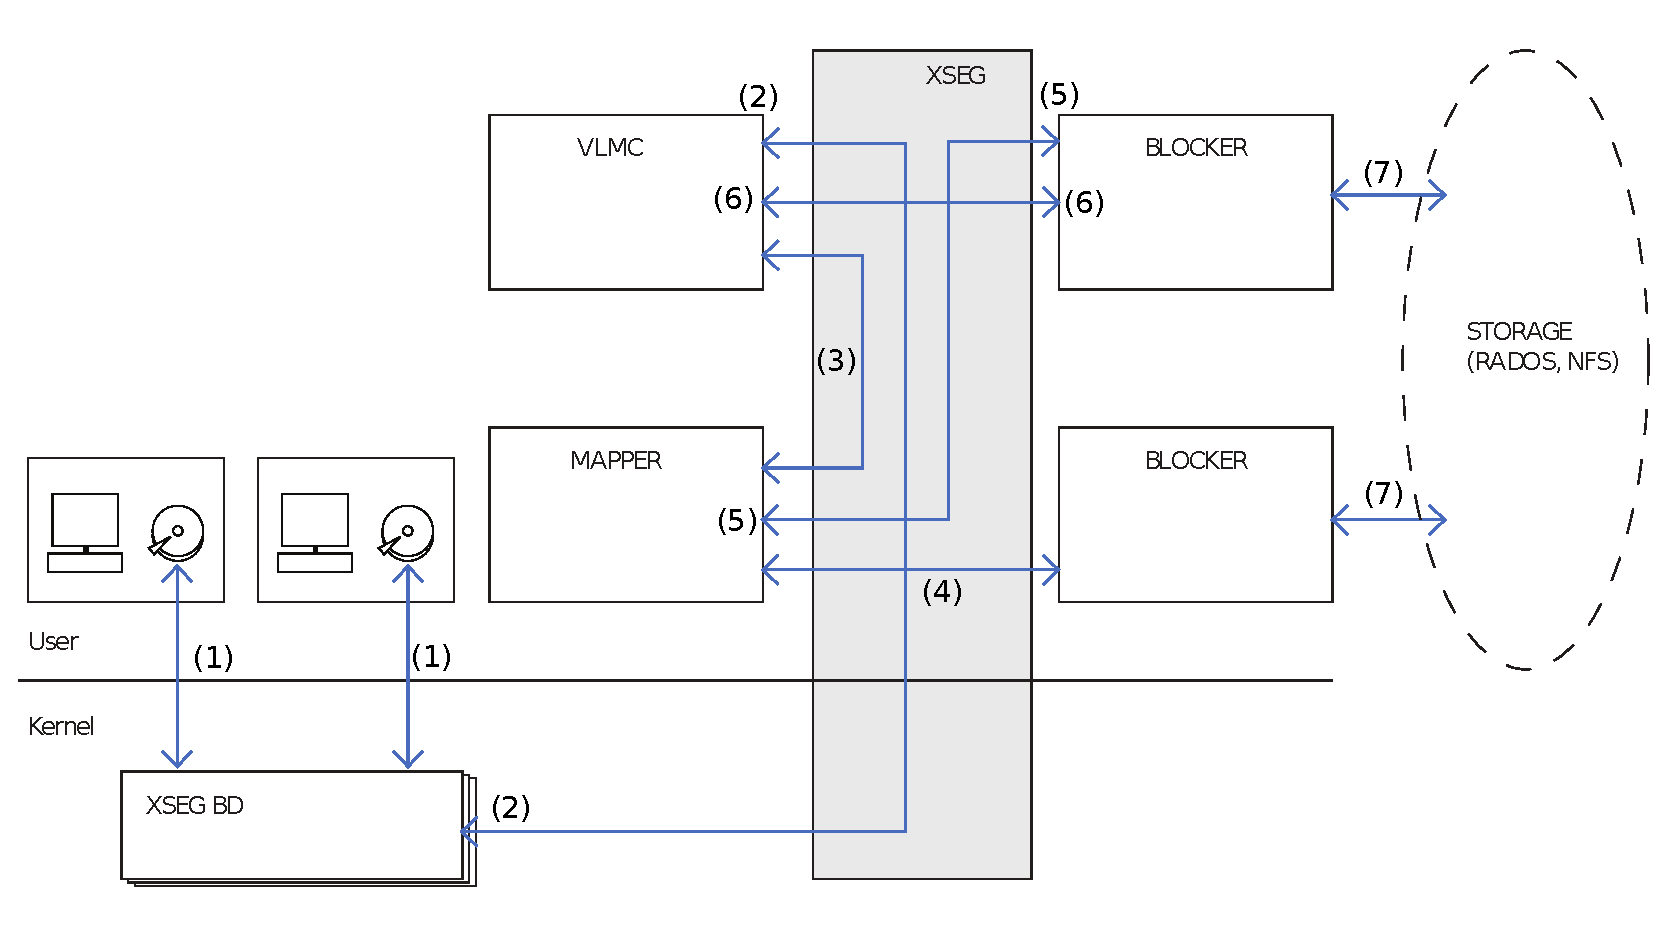
\includegraphics[width=\columnwidth]{images/new_sxima_numbered.pdf}
		\end{column}
	\end{columns}
	\note[item]{Και εδώ βλέπουμε τα διακριτά κομμάτια κώδικα που υλοιποιούν τα 
		παραπάνω και τα οποία θα συζητήσουμε ευθύς αμέσως}
\end{frame}

\begin{frame}{Xcache design}
	\centering\includegraphics<1>[height=0.6\textheight]{images/xcache-design.pdf}
	\centering\includegraphics<2>[width=\textwidth]{images/xcache-entry.pdf}

	Xcache is responsible for: 1) entry indexing, 2) entry eviction, 3) 
	concurrency control

	\note[item]{Αυτό είναι το xcache, που είναι υπεύθυνο για την
		\begin{itemize}
			\item Indexing των αντικειμένων
			\item Eviction αντικειμένων από την cache με τη χρήση LRU
			\item Χειρισμό προσβάσεων από πολλαπλά threads
		\end{itemize}
	}
	\note[item]{Έχουμε δυο hash table, το καθένα με το δικό του lock, ένα χώρο 
		που αποθηκεύονται οι εγγραφές των αντικειμένων και μόνο (όχι τα 
		δεδομένα, προσοχή) και μια στοίβα όπου κρατιούνται indexes των 
		ελεύθερων entries, προστατευόμενη από ένα lock.}
	\note[item]{To ένα hash table <αυτό> που κρατάει τα ονόματα των cached 
		αντικειμένων.}
	\note[item]{To άλλο hash table κρατάει τα ονόματα των evicted αντικειμένων 
		έως ότου ελευθερωθούν ή ξαναγίνουν cached.}
	\note[item]{Ο αποθηκευτικός τους χώρος είναι preallocated και είναι <αυτό>.  
		Σε αυτό το χώρο, η αναφορά γίνεται με δείκτες.}
	\note[item]{Τα ελεύθερα entries είναι στη στοίβα αυτή.}
	\note[item]{\click}
	\note[item]{Κάθε item έχει ένα reference counter για να ξέρουμε πόσοι το 
		χρησιμοποιούν, όνομα, και δείκτες για την lru}
	\note[item]{Συγκεκριμένα, στο παράδειγμα αυτό, το entry αυτό είναι το 
		τελευταίο LRU, αυτό είναι το MRU κτλ. χέρι στον πίνακα}
	\end{frame}

\begin{frame}{Xworkq design}
	\centering\includegraphics<1>[width=\textwidth]{images/xworkq-design.pdf}

	Xworkq is responsible for concurrency control
	\note[item]{xworkq υπεύθυνο για την ασφαλή επεξεργασία των δεδομένων 
		ενός αντικείμενου.}
	\note[item]{Δεν μπορεί πάνω από ένας να πειράζει τα data ενός thread. Το 
		spinning είναι αργό, όλοι τοποθετούν μια δουλειά σε μια ΟΥΡΑ, ένας την 
		εκτελεί.  Έτσι, ένα thread εκτελεί μια δουλειά και τα υπόλοιπα είναι 
		ελεύθερα να κάνουν κάτι πιο χρήσιμο}
	\end{frame}

\begin{frame}{Xwaitq design}
	\centering\includegraphics<1>[width=\textwidth]{images/xwaitq-design.pdf}

	Xwaitq is responsible for deferred execution
	\note[item]{xwaitq υπεύθυνο για την υπό συνθήκη εκτελεση εργασιών}
	\note[item]{Αν π.χ. μας τελειώσει ο χώρος, δεν μπορούμε να περιμένουμε 
		σύγχρονα. To thread μπορεί να τοποθετήσει μια δουλειά και μετά 
		να εκτελέσει κάτι άλλο}
\end{frame}

\begin{frame}{Bucket pool}
	Cached divides an object (commonly 4MB) to buckets (commonly 4KB) which are 
	always fully written.
	When an object is indexed however, it does not have immediate access to all 
	of its buckets because:
	\begin{itemize}
		\item RAM is limited
		\item Most objects would probably be half-written
	\end{itemize}
	\note[item]{Σπάμε τα objects (τυπικά έχουν 4MB) σε buckets (τυπικά των 
		4KΒ).  Άρα κάθε object έχει 1024.}
		\note[item]{Το ότι κάνουμε index ένα object δε σημαίνει ότι αυτομάτως 
			έχει και τα 1024 buckets}
	\note[item]{Δεν υπάρχει τόση RAM και άλλωστε πολλά objects μπορεί να είναι 
		μισό-γραμμένα}
	Ideally, we want to:
	\begin{itemize}
		\item Decouple the objects from their data
		\item Cache unlimited objects but put a limit on their data
	\end{itemize}
	\note[item]{Ιδανικά θέλουμε να διαχωρίσουμε την καταχώρηση/όνομα του 
		αντικειμένου από τα δεδομένα του. Δυνητικά θα μπορούμε να καταχωρούμε 
		πάρα πολλά αντικείμενα αλλά θα έχουμε μικρότερο cache size}

	Solution:
	\begin{itemize}
		\item Preallocated data space (=cache size) separated in buckets
		\item Every object requests a range of buckets for a request
		\item When an object is evicted, its buckets are reclaimed
	\end{itemize}
	\note[item]{Preallocated χώρος, όλοι παίρνουν indexes από αυτό (Θυμίζει 
		xcache, ΠΕΣ για WAITQ}
\end{frame}

\begin{frame}{Other important cached tasks}

	Several other key-tasks are:
	\begin{itemize}
		\item Book-keeping
		\item Cache write policy
		\item Asynchronous task execution
		\item Data propagation
	\end{itemize}
	\note{Το cached είναι επίσης επιφορτισμένο και με άλλες δουλειές όπως:
		\begin{itemize}
			\item Κρατάει στατιστικά (πόσα entries είναι dirty, 
				πόσα buckets έχει κάνει allocate ένα entry
			\item Εφαρμόζει writeback/writethrough πολιτική
			\item Φρόντίζει ώστε οι εργασίες να μπορούν να γίνουν 
				ασύγχρονα
			\item Και φυσικά φροντίζει τα δεδομένα να γράφονται 
				σωστά στο storage
		\end{itemize}
	}
\end{frame}

\begin{frame}{Cached flow}
	\includegraphics<1>[height=0.8\textheight]{images/cached-design2.pdf}
	\includegraphics<2>[height=0.8\textheight]{images/cached-design-comp2.pdf}

	\note[item]{Εδώ παίζεις με τα slides}
	\note[item]{Θα παρουσιάσουμε πολύ γρήγορα τη ροή ενός αιτήματος στον 
		cached}
	\note[item]{Έρχεται request, το κάνουμε index, μπαίνουμε στη workq και 
		πειράζουμε τα δεδομένα του και ανάλογα το cache policy το 
		γράφουμε πίσω στον blocker αλλιώς τελειώσαμε}
	\note[item]{Optional σεναρια:
		\begin{itemize}
			\item Αν γίνει ένα eviction, πρέπει να γράψουμε τα 
				δεδομένα του πίσω με ασφάλεια. Επειδή το 
				αντικείμενο μπορει να καταχωρηθεί, να μπει και 
				να ξαναβγεί, πρέπει να είμαστε προσεκτικοί
			\item Αν ξεμείνουμε από πόρους (χώρο στο hash table, 
				buckets κτλ, πρέπει να συνεχίσουμε μονο όταν 
				μπορούμε
		\end{itemize}
	}
\end{frame}

\chapter{Implementation of cached}\label{ch:cached-implementation}

In the previous chapter, we have discussed in length the design of cached and 
its components. In this chapter, we will present how the above design has been
implemented. To aid us in this task, we will use code snippets from cached, and 
xcache and we will comment where necessary.

More specifically, Section \ref{sec:xcache-imp} presents the implementation of 
xcache, the main cached component. Next, section \ref{sec:cached-imp} presents 
the implementation of cached and demonstrates the structures and functions that 
are used.

\section{Implementation of xcache}\label{sec:xcache-imp}

For this section, we will attempt to provide a top-down view of the xcache 
implementation, starting from the functions that xcache exposes to peers and 
moving on to the more intrinsic details, such as the concurrency control.

\subsection{xcache initialization}

In order to use xcache, the peer must first initialize an xcache structure 
using \texttt{xcache\_init}, which can be seen in Listing 
\ref{lst:xcache-init.h}.

\ccode{Definition of \texttt{xcache\_init}}{xcache-init.h}

\texttt{xcache\_init} requests the following information from the peer:

\begin{description}
	\item[cache:] Simply, an allocated xcache struct.
	\item[xcache\_size:] The number of objects xcache will index.
	\item[ops:] The trigger functions for xcache's event hooks.
	\item[flags:] Optional flags that tune the following two things:
		\begin{enumerate}
			\item The LRU algorithm. For the cached implementation, 
				we use the O(1) LRU, but xcache also allows to 
				use two more LRU algorithms, a binary heap 
				(O(log(N))) or an LRU array (O(N)).
			\item The usage of the hash table for evicted entries.  
				Although our cached implementation relies 
				heavily on it, this does not account for all 
				the other peers that use xcache and by default 
				is not used.
		\end{enumerate}
	\item[priv:] A pointer (void *) to a structure that will be returned 
		when an event hook is triggered. As most priv fields, it is 
		irrelevant to the xcache struct and relevant only to the top 
		caller. We initialize it with the peer struct.
\end{description}

The purpose of xcache\_init is to process the above data, populate the xcache 
struct and create the necessary entities, such as the hash table, the cache 
entries etc. On Listing \ref{lst:xcache-struct.h}, we can view the xcache 
struct and its respective fields.

\ccode{Main \xcache struct}{xcache-struct.h}

Each of the above \xcache struct fields is used to implement a design feature 
that has already been discussed in Section \ref{sec:xcache-design}. In the 
following sections, we will revisit these design features and present their 
implementation.

\subsection{Cache entry preallocation}

When xcache is initialized, it preallocates the necessary cache entries. The 
relevant xcache fields for this purpose can be seen in Listing 
\ref{lst:xcache-prealloc.h}.

\ccode{\xcache struct fields relevant to preallocated 
	entries}{xcache-prealloc.h}

The \textbf{size} field is the number of entries. The \textbf{free\_nodes} is a 
stack where all entry indexes are initially pushed and subsequently popped when 
a new entry is inserted. Finally, \textbf{nodes} is the space allocated for the 
cache nodes and where the entry indexes point to.

Moreover, the definition of the \texttt{xcache\_entry} struct is shown in 
Listing \ref{lst:xcache-entry.h}.

\ccode{The \texttt{xcache\_entry} struct}{xcache-entry.h}

We will comment briefly on the relevant \texttt{xcache\_entry} fields for this 
section, which can be seen in Listing \ref{lst:xcache-entry-prealloc.h}. The 
rest of the fields will be discussed in the following sections.

\ccode{\texttt{xcache\_entry} fields, relevant to 
	preallocation}{xcache-entry-prealloc.h}

The description of the fields follows:

\begin{description}
	\item[ref:] The reference count of the entry, initially set to zero.
	\item[state:] The state of the entry. It can either be ACTIVE or 
		EVICTED and is initially set to the first.
	\item[name:] The name of the entry. Since we cannot know its length 
		beforehand, we allocate as much space as possible, typically 
		256 characters. During initialization, the entry name is 
		cleared out of junk values.
	\item[priv:] The private contents of the cache entry. On 
		initialization, the cache node creation hook is triggered and 
		cached initializes the private contents of cache entry with its 
		data (more on Section \ref{sec:xcache-hooks-imp})
\end{description}

\begin{comment}
	The rest willwhaLet's start by listing what \texttt{xcache entry} 
	consists of.  First of all, it must have a name.  Since we preallocate 
	the entries and cannot know in runtime their length, we must allocate 
	as much space as possible. The \texttt{char name[XSEG\_MAX\_TARGETLEN + 
		1]} field, which is 256 characters long, is long enough to hold the 
	target's name.  Also, as we have mentioned in Section 
	\ref{sec:entry-prealloc-design}, xcache must be agnostic of the cache 
	contents.  To this end, we use the generic \texttt{void *priv} field as 
	a pointer to the actual entry content.  The rest of the fields will be 
	explained in the following chapters.

	Let's continue now with the fields of Listing \ref{lst:xcache-prealloc.h}.  
	Since we preallocate the entries using \texttt{malloc}, they take up a 
	contiguous space in memory.  The start of this space is the where the 
	\texttt{*nodes} field points to. The \texttt{free\_nodes} field works similarly 
	to the free\_entries field in Section \ref{sec:get-req-archip} i.e. it is a 
	stack where indexes to unused nodes are pushed. These indexes will be seen in 
	various code excerpts in this chapter and have a specific name, 
	\texttt{xcache\_handler}\footnote{\#define xcache\_handler uint64\_t}.
\end{comment}

\subsection{Cache entry initialization}

Before a peer can index a new entry, it must first allocate it from the cache 
entry pool and then initialize it. Xcache has a special function for this 
purpose, which can be seen in Listing \ref{lst:xcache-alloc-init.c}.

\ccode{Allocation/initialization function for 
	\texttt{xcache\_entry}}{xcache-alloc-init.c}

This function attempts to claim an \texttt{xcache\_entry} index from the
\texttt{free\_nodes} stack.  Then it initializes it with the name given by the 
peer.  Moreover, it triggers the cache entry initialization hook which cached 
uses to further initialize the entry.

An added benefit of this function is that it doesn't need to acquire the main 
cache lock, so it does not slow down the indexing functions that rely on that 
lock.

\subsection{Cache entry indexing}

This is the core feature of xcache. In Listing \ref{lst:xcache-index.h}, we 
present the fields of the xcache struct that are relevant to the indexing task.

\ccode{xcache struct fields relevant to entry indexing}{xcache-index.h}

As we have mentioned in Section \ref{sec:xcache-index-design}, we utilize two 
hash tables, one for the active entries and one for the evicted entries. These 
hash tables can be accessed from xcache and are the \texttt{*entries} and 
\texttt{*rm\_entries} fields respectively.

More importantly, in Listing \ref{lst:xcache-index.c} we can see the functions 
that are related to indexing and xcache exposes to the peer:

\ccode{Indexing functions}{xcache-index.c}

All of these functions need a pointer to the xcache struct. Here's a brief 
description of them:

\begin{description}
	\item[xcache\_lookup:]
		Takes the target's name as an argument and searches for it in 
		cache.\\
		Returns on failure: NoEntry\\
		Returns on success: the requested handler.\\
		\textbf{Note:} Looks only in \texttt{entries}.
	\item[xcache\_insert:]
		Takes the handler of an allocated entry as an argument and uses 
		it to index that entry.\\
		Returns on failure: NoEntry.\\
		Returns on success:
		\begin{inparaenum}[i)]
		\item the same handler or,
		\item if the same entry already exists in cache, the handler of that 
			entry.
		\end{inparaenum}\\
		\textbf{Note:} It looks up first if the entry exist in 
		\texttt{entries} or \texttt{rm\_entries}. The later case can 
		lead to re-insertions.
		\item[xcache\_remove:]
			Takes the handler of an allocated entry as an argument and uses 
			it to remove that entry.\\
			Returns on failure: -1.\\
			Returns on success: 0.\\
			\textbf{Note:} Removes only active entries .
\end{description}

Moreover, in Listing \ref{lst:xcache-entry-index.h}, we show the 
\texttt{xcache\_entry} fields that are related to indexing, and comment on how 
they are used by each function.

\ccode{xcache entry struct relevant indexing}{xcache-entry-index.h}

\begin{description}
	\item[ref:] The reference counter of an object is increased on lookups 
		and inserts, since it is essentially referenced in these 
		operations.
	\item[state:] The state of the entry is set to ACTIVE.
	\item[older/younger]: These fields show the neighbors of the entry in 
		the LRU queue. The LRU queue is sorted by reference time order, 
		so the neighbors are essentially the entries that have been 
		referenced right before and right after our entry.
\end{description}

\subsection{Entry eviction}\label{xcache-evict-imp}

The relevant fields for this purpose can be seen in Listing 
\ref{lst:xcache-evict.h}.

\ccode{\xcache struct fields for eviction}{xcache-evict.h}

As we have mentioned in Section \ref{sec:xcache-eviction-design}, we resort to 
eviction when the cache is full and new entries can't be inserted. By xcache 
policy, we evict the least recently used entry. The necessary fields for the 
doubly-linked list that we maintain for this purpose can be seen below:

\ccode{Doubly-linked LRU list}{xcache-dlist.h}

The last entry of the list (oldest) is usually the LRU. When an object is 
referenced, it can be instantly transferred to the head of the list (MRU), 
since we know its position via the hash table (alternatively, we would need to 
search all entries, which would require O(N) time).

Another feature of this LRU queue is that it doesn't require timestamps, so we 
can avoid the unnecessary system call.

When we have found out which entry to evict, we migrate it from the hash table 
of active entries to the hash table of evicted entries. This process is 
explained in depth in Section \ref{sec:xcache-eviction-design}.

Finally, when a cache entry is evicted from the hash table, it triggers the 
cache entry eviction hook.

\begin{comment}
\begin{itemize}
	\item Insert a new entry to the LRU list
	\item Evict the LRU entry
	\item Update an entry's access time (i.e. mark it as MRU)
	\item Remove an arbitrary entry
\end{itemize}

Lets explain these fields a bit:

\begin{description}
	\item[lru:] Obviously, it's the least recently used entry. It can be 
		considered as the one end of the doubly linked list.
	\item[mru:] The entry that has just been used. It can be considered as 
		the other end of the doubly-linked list
	\item[younger:] This entry-specific field points to an entry used right 
		after our entry was used.
	\item[older:] Same as "younger", it points to the entry that has been 
		used right before our entry was used.
\end{description}

Finally, as we have explained in Section \ref{sec:xcache-evict-design}, the 
eviction internals should normally not bother the user. However, if the user 
wants to, \xcache exposes the following functions:

\begin{description}
	\item[xcache\_evict\_lru:] The name says it all, it evicts the recently 
		used item.
	\item[xcache\_peek\_and\_get\_lru:] This function allows the user to 
		atomically take a peek on the Least Recently Used entry and also 
		update its refcount.
\end{description}
\end{comment}

\subsection{Entry reinsertion}

We have seen in the previous section how an active entry is evicted. However, 
what happens when xcache receives a request for an evicted entry which hasn't 
been freed yet? 

In this case, the entry migrates back to the hash table of active entries.  
Also, its reference counter is incremented by 1, since the xcache can now 
reference this entry again.

The advantage of reinsertion is that we do not stall until the evicted entry 
has flushed all its data and instead, we can use it immediately.

\subsection{Concurrency control}\label{sec:xcache-conc-imp}

Concurrency control is an extremely important aspect of xcache, if we want to 
utilize an SMP system to its full potential. Although parts of the concurrency 
control have already been discussed in previous sections, in this section, we 
will provide an in-depth explanation of how xcache implements them.

The relevant fields for concurrency control can be seen in Listing 
\ref{lst:xcache-conc.h}, both for the xcache and \texttt{xcache\_entry} 
structs.

\ccode{Concurrency control fields}{xcache-conc.h}

There are three main techniques xcache uses for concurrency control. The first 
one is the usage of locks, the second one is reference counting and the third 
one is the tracking of parallel puts to an entry, a more esoteric method that 
counters the ABA problem.

\subsubsection{Locking}\label{sec:xcache-lock-imp}

With xcache, we have tried not to use a BKL
\footnote{BKL stands for Big Kernel Lock and was a giant lock in kernel space 
	that inhibited the performance of SMP systems and remained until the 
	late stages of the 2.6 Linux kernel}
type of lock, but instead use many smaller ones.

Specifically, we have used:
\begin{enumerate}
	\item a lock that protects the cache entry pool from concurrent 
		accesses. Since the only operation this lock protects is the 
		push and pop of cache entry indexes, we expect that there will 
		be no contention on it.
	\item the \texttt{lock} lock, as seen in the xcache struct, which is 
		our main lock as it protects the hash table of active entries 
		(\texttt{entries}) from concurrent accesses. This lock is used 
		during lookups, inserts and evictions, so it is the lock with 
		the most contention.
	\item the \texttt{rm\_lock}, which protects the hash table of evicted 
		entries (\texttt{rm\_entries}) from concurrent accesses and is 
		used during insertions, evictions and puts.
	\item a lock in every entry, which is specifically used when an entry 
		is put.
\end{enumerate}

Of major importance is also the issue of deadlocking. More specifically, during 
inserts or evictions, we need to have access on both hash tables. If a thread 
acquired the lock of one hash table and another thread acquired simultaneously 
the lock of the other, we would have a deadlock since both would need a lock 
that the other thread has.

To this end, xcache strictly acquires the locks in the following order: 
\texttt{lock} --> \texttt{rm\_lock} --> entry lock. With this policy we are 
sure that there will be no deadlocks.

\subsubsection{Reference counting}\label{sec:xcache-refcount-imp}

Each cache entry has a volatile uint64\_t field which is atomically get and 
put. The type is volatile to inform the compiler that it might be changed 
outside the current execution context and therefore do not cache it in a 
register.

Furthermore, the atomic gets and puts are executed using the GCC 
builtins\cite{gcc-atomic} which are shown in Listing \ref{lst:xcache-atomic.c}.

\ccode{Atomic operations of GCC}{xcache-atomic.c}

The refcount model in xcache should be familiar to most people:

% Turn this to figure
\begin{itemize}
	\item When an entry is inserted in cache, xcache holds a reference to 
		it (ref = 1).
	\item Whenever a new lookup for this cache entry succeeds, the reference 
		is increased by 1 (ref++)
	\item When a request has been completed and no longer needs the entry, 
		the reference is decreased by 1. (ref--)
	\item When a cache entry is evicted by xcache, its ref is decreased by 
		1, since it no longer holds a reference to it. (ref--)
\end{itemize}

Moreover, some common refcount cases are:

\begin{itemize}
	\item active entry with pending jobs (ref > 1)
	\item active entry with no pending jobs (ref = 1)
	\item evicted entry with pending jobs (ref > 0)
	\item evicted entry with no pending jobs (ref = 0)
\end{itemize}

\begin{comment}
\begin{table}
	\centering
	\begin{tabular}{ | l | l | }
		\hline
		Case & Refcount \\ \hline \hline
		active entry with pending jobs & ref > 1 \\ \hline
		active entry with no pending jobs & ref = 1 \\ \hline
		evicted entry with pending jobs & ref > 0 \\ \hline
		evicted entry with no pending jobs & ref = 0 \\ \hline
	\end{tabular}
	\caption{Reference counting of xcache}
	\label{tab:refcount}
\end{table}
\end{comment}

Unlike most refcount cases, however, the entry is not put when its refcount 
drops to zero. The reason is that the entry can be reinserted at any time. In 
the following section, we explain how we have handled that case.

\subsubsection{Parallel puts}

The scenario of putting the entry has proved the most tricky one and deserves 
its own section in the concurrency control implementation.

For this scenario, we aimed to avoid the usage of our two biggest locks: 
\texttt{lock} and \texttt{rm\_lock}. Avoiding the first one was easy since the 
hash table of active entries was not used. However, the same did not hold true 
for the \texttt{rm\_lock}, since the evicted entry must be reliably removed 
from the hash table of evicted entries. However, we have managed to reduce its 
usage to the absolute minimum.

The put procedure is the following:

\begin{enumerate}
	\item We decrement the refcount of the entry.
	\item If the refcount is more than zero, we leave.
	\item Else, we proceed by triggering the on\_finalize hook. With this 
		hook, the peer is given a chance to increment the refcount of 
		the entry if it deems it necessary (e.g. the entry is dirty).
	\item After we have returned from this hook, we check if the refcount 
		is zero.  This time, we use the \texttt{rm\_lock} to prevent 
		reinsertions and remove the entry from the hash table of 
		evicted entries.
	\item If the refcount is not zero, then someone in the meantime has 
		reinserted the entry and we can safely leave.
	\item Else, we remove the entry.
\end{enumerate}

This procedure looks simple at first glance. However, looks are deceiving and 
so is the ABA problem. In our case, consider the following:

\begin{enumerate}
	\item Tread 1 \textrightarrow\ evicts a clean entry \textbf{(ref 0)}
	\item Thread 1 \textrightarrow\ triggers the on\_finalize hook
	\item Thread 2 \textrightarrow\ reinserts the entry \textbf{(ref 2)}
	\item Thread 2 \textrightarrow\ makes the entry dirty and then puts it 
		\textbf{(ref 1)}
	\item Thread 3 \textrightarrow\ evicts the now dirty entry           
		\textbf{(ref 0)}
	\item Thread 1 \textrightarrow\ checks if the reference count is zero 
		and removes the entry
	\item Thread 3 \textrightarrow\ triggers the on\_finalize hook, 
		increments the refcount of the entry and issues a flush for its 
		contents
		\textbf{(ref 1)}
\end{enumerate}

Although the final refcount is correct, the entry has been removed midway the 
put procedure. The fault in our logic was that we expected that, if the 
refcount is zero before and after the on\_finalize hook, we could safely remove 
the entry. This is commonly referred to in the bibliography as the "ABA 
problem"\cite{aba}. Generally, it occurs when a thread reads twice a "guard" 
variable and gets the same value, but is unaware of the fact that it has 
changed in between these two checks.

The ABA problem is mostly encountered in lock-free structures and since xcache 
does not aim to be one of them, we can simply lock the put procedure with the 
\texttt{rm\_lock}. However, this can have a performance impact, especially if a 
peer plugs a slow on\_finalize trigger function.

We have chosen instead to use an extra \texttt{xcache\_entry} field called 
\texttt{parallel\_puts}.  This number is incremented when a thread enters the 
put function and has dropped the reference of the object to zero i.e. between 
steps one and two. This way, we can also check during step five the number of 
parallel puts if and leave if it is more than one.

\subsection{Event hooks}\label{sec:xcache-hooks-imp}

The hooks that xcache provides to users are stored in an xcache\_ops struct 
that can be seen in Listing \ref{lst:xcache-hooks.h}.

\ccode{xcache\_ops struct}{xcache-hooks.h}

The design of these hooks has been presented on Section 
\ref{sec:xcache-hooks-design}. The functions that are attached to each hook 
return two values:
\begin{inparaenum}
\item the private field of xcache (the peer structure in our case) and
\item the cache entry's private data (the object in our case) for which the 
	hook was triggered.
\end{inparaenum}

\section{Implementation of cached}\label{sec:cached-imp}

In this section, we will present the implementation of cached. A presentation 
of the design of cached is provided in Section \ref{sec:cached-design}.  
Similarly to xcache, we will begin with the initialization process, we will 
continue with the request handling and finish with presenting the challenges we 
faced and the solutions we implemented.

\subsection{Cached initialization}\label{sec:cached-init-imp}

We have mentioned in the previous chapters that cached can be multi-threaded, 
have different write policies, maximum number of objects, cache size etc. All 
these variables are given from command-line and used during cached 
initialization. The necessary arguments are:

\begin{itemize}
	\item Number of threads
	\item Max objects to cache
	\item Total cache size
	\item Object size
	\item Bucket size
	\item Blocker port
	\item Write policy
\end{itemize}

and the cached structure that is initialized is presented in Listing 
\ref{lst:cached.h}. 

\ccode{Main cached struct}{cached.h}

Moreover, on cached initialization we also initialize xcache as well as the 
necessary xworkqs and xwaitqs.

Some of the above cached fields are the same with the command-line arguments 
and are self explanatory. We will briefly comment on the less obvious fields, 
which will be discussed in length in their respective sections.

\begin{description}
	\item[cache:]
		The initialized xcache struct is stored here.
	\item[max\_req\_size:]
		The maximum request size that can be sent to the blocker.
	\item[workq:]
		A lockless xworkq where non-critical jobs from threads who are 
		in a critical section are enqueued.
	\item[pending\_waitq:]
		An xwaitq for jobs that need to allocate a cache entry to.
		continue
	\item[bucket\_waitq:]
		An xwaitq for jobs that need to allocate a bucket to continue.
	\item[req\_waitq:]
		An xwaitq for jobs that need to allocate a request to continue.
	\item[bucket\_data:]
		The bucket pool of cached, Its size is the total\_size of 
		cached.
	\item[bucket\_indexes:]
		The stack where bucket indexes are pushed.
\end{description}

Furthermore, during the xcache initialization that takes place inside the 
cached initialization, the cached node initialization hook is triggered and 
cached can create its objects, which are as many as the max objects.  
Programmatically, cached objects are called "ce"s and their structure can be 
seen in Listing \ref{lst:ce.h}.

\ccode{Cached entry struct}{ce.h}

The explanation of the above fields follows:

\begin{description}
	\item[status:] The object status, as seen in Section 
		\ref{sec:cached-states-design}.
	\item[lock:] The lock for the ce's and its buckets' data.
	\item[workq:] The xworkq that is used for concurrency control over 
		parallel access to the ce's and its buckets' data. It uses the 
		aforementioned lock.
	\item[pending\_waitq:] The xwaitq that is used when a request cannot be 
		executed due to the ce's state. It will allow job executions 
		only when the object is not in FLUSHING state.
\end{description}

We have intentionally left out the bucket related fields that will be discussed 
in length in Section \ref{sec:cached-bucket-imp}.

\subsection{Bucket pool}\label{sec:cached-bucket-imp}

The initialization of the bucket pool is covered in Section 
\ref{sec:cached-init-imp}. In this section, we will explain how this bucket 
pool is connected with the buckets of each ce.

When the cache node initialization hook is triggered, the ce's buckets are 
initialized. Essentially, this means we do (once only) the following:

\begin{enumerate}
	\item First, we allocate an array of struct buckets. The array has
		\texttt{buckets\_per\_object} length, which is typically 1024 
		(4MB objects / 4KB bucket size). The struct bucket is a very 
		simple struct and is presented in Listing 
		\ref{lst:bucket.h}.
		
		\ccode{Bucket implementation}{bucket.h}

	\item Second, we allocate two more arrays, the  
		\texttt{bucket\_alloc\_status\_counters} array and the
		\texttt{bucket\_data\_status\_counters} array, whose length is 
		the number of allocation states (2) and data states (5) 
		respectively.
	\item Third, we initialize each bucket's allocation state to FREE and 
		data state to INVALID. The allocation and data state are stored 
		in the \texttt{flags} section of struct bucket, which is 
		actually a custom bit-field with support for variable field 
		lengths.
	\item Finally, we initialize all the counters to zero, besides the 
		allocation counter for FREE buckets and the data counter for 
		INVALID buckets, which are set to \texttt{buckets\_per\_object} 
		(1024).
\end{enumerate}

None of the above operations, however, interact with the bucket pool. This is 
because we do not initially attach the bucket indexes to the ce's buckets.

The way buckets are attached to the object is analogous to the way a function 
maps to its address space a large memory chunk which has previously allocated; 
the chunk is internally divided to smaller chunks and when the function 
attempts to "touch" them, it is trapped and then the buckets are mapped to the 
function's address space.

Similarly, when cached accepts a request for a target, the request's range is 
translated to bucket range. If any of the buckets within that range are not 
attached to the ce, the request is "trapped" and the needed buckets are claimed 
from the bucket pool.

Finally, the bucket claiming and release procedure is the following:
\begin{enumerate}
\item We pop a bucket index from the \texttt{bucket\_indexes} stack,
\item We translate it to the actual data pointer and store it to the 
	\texttt{data} field of the struct bucket,
\item When the bucket is released, we translate the data pointer back to the 
	bucket index
\item We push the bucket index back to the bucket pool.
\end{enumerate}

\subsection{Request handling}

Cached uses the request polling scheme that we have described in Section 
\ref{sec:arch-poll}, with the addition of the following:

\begin{enumerate}
	\item Checks for the state of the bucket pool. If the bucket pool has 
		been depleted, we force flush the LRU entry to acquire its 
		buckets.
	\item Periodic signals to the cached's xworkq.
\end{enumerate}

When a request is accepted/received, it is forwarded to the appropriate handle 
function based on its xcache operation type.

More specifically, for accepted (new) requests, we index the request target 
(object) and store its xcache handler on the request's cache-io and we proceed 
according to its operation type. For received requests, the request's cache-io 
holds the xcache handler for the object, so we can proceed immediately 
according to its operation type. The way the request is handled next is 
documented in Section \ref{sec:cached-flow-design}.


\section{Cached evaluation}

\begin{frame}{Benchmark methodology}
We have conducted exhaustive benchmarks.\\
They are separated in three categories:

\begin{itemize}
	\item Comparison between cached over RADOS and RADOS solely
		\begin{itemize}
			\item Peak behavior
			\item Sustained behavior
		\end{itemize}
	\item Internal measurement of cached
		\begin{itemize}
			\item Indexing mechanism overhead
		\end{itemize}
	\item Evaluation of VM/Archipelago
\end{itemize}
\spc
Note: sosd refers to the blocker driver of Archipelago

\note{Οι μετρήσεις μας είναι εκτενείς και χωρίζονται σε τρεις κατηγορίες:
	\begin{itemize}
		\item Σύγκριση performance του cached και rados για workloads 
			μικρότερα και μεγαλύτερα του cache size
		\item Αξιολόγηση εσωτερικών κομματιών του cached (συγκεκριμένα overhead 
			του indexing μηχανισμού
		\item Μετρήσεις του Αρχιπελάγους για ένα πραγματικό VM
	\end{itemize}

	Στις επόμενες μετρήσεις, όπου sosd εννοούμε rados. Επίσης, όλα είναι random 
	i/o

	Σημείωση, τρίτη κατηγορία είναι πολύ σημαντική. Καταφέραμε να σηκώσουμε 
	πραγματικό VM με cached. Αυτό είναι το highlight της διπλωματικής
}

\end{frame}

\begin{frame}{Cached/sosd comparison - peak behavior}
	\begin{columns}[t]
		\begin{column}{.5\textwidth}
			Write bandwidth
			\makebox[\textwidth]{
				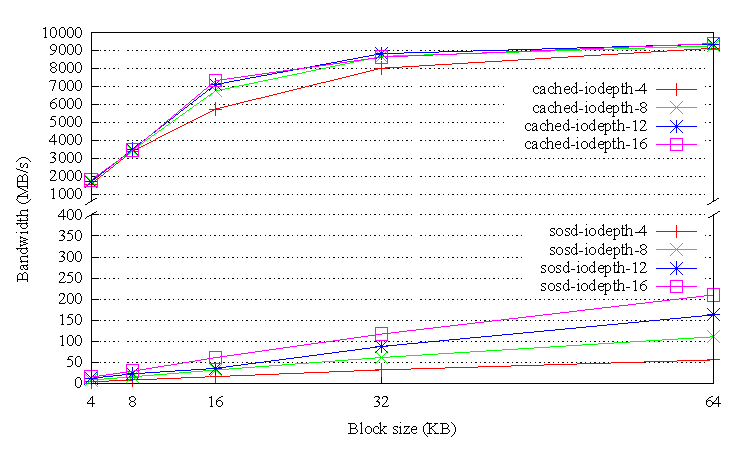
\includegraphics[width=\columnwidth]{images/bw-write-comp-lie.pdf}
			}
			Constants:
			\begin{itemize}
				\item cached has 4 threads
				\item workload size less than cache size
			\end{itemize}
		\end{column}
		\begin{column}{.5\textwidth}
			Read bandwidth
			\makebox[\textwidth]{
				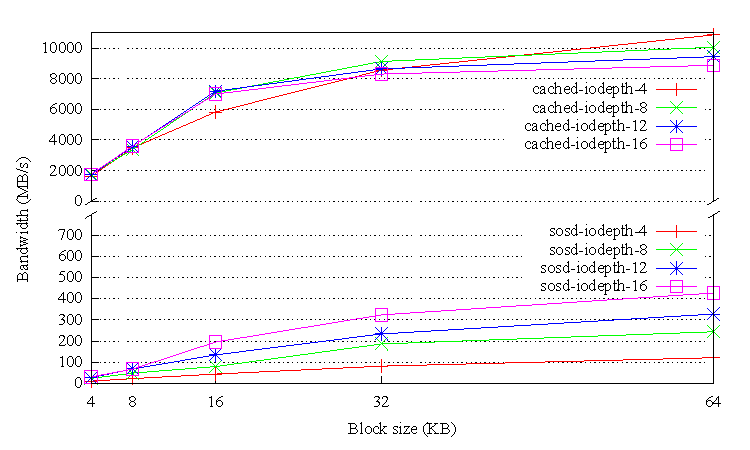
\includegraphics[width=\columnwidth]{images/bw-read-comp-lie.pdf}
			}
			Variables:
			\begin{itemize}
				\item block size [4KB - 64KB]
				\item parallel requests [4 - 16]
			\end{itemize}
		\end{column}
	\end{columns}

	\note[item]{Ας περιγράψουμε το benchmark μας. Στείλαμε καρφωτά στους peers 
		requests των...}
	\note[item]{Το iodepth είναι ο αριθμός των παράλληλων requests}
	\note[item]{Σημεία προσοχής:Για μικρά writes είμαστε έως 100x 
		γρηγορότεροι ενώ για μεγάλα έως 200x. }
	\note[item]{O cached μετά τα 16ΚΒ δεν κάνει scale - χτυπάμε το 
		bandwidth της RAM}
	\note[item]{Έχουμε lock contention, δε θα έπρεπε να αυξάνεται η 
		ταχύτητα για μεγάλα blocks και δεν αυξάνεται η ταχύτητα με 
		parallel requests}
	\note[item]{Lock contention είναι ότι δεν κάνουμε scale με πολλά threads 
		για μικρά block sizes}
\end{frame}

\begin{frame}{Cached/sosd comparison - peak behavior}
	\begin{columns}[t]
		\begin{column}{.5\textwidth}
			Write latency
			\makebox[\textwidth]{
				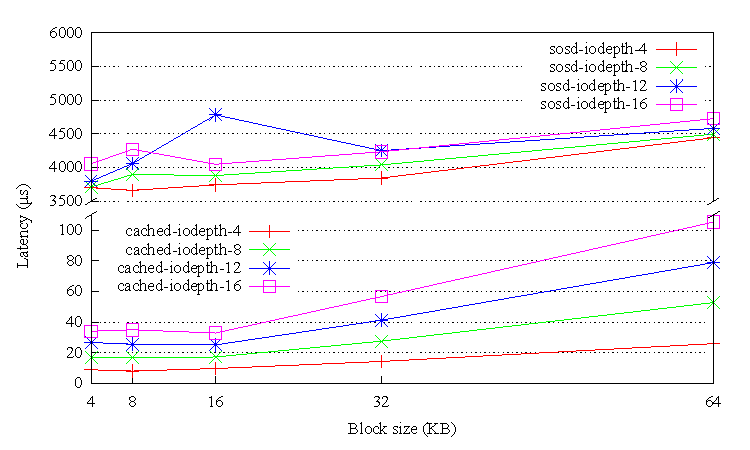
\includegraphics[width=\columnwidth]{images/lat-write-comp-lie.pdf}
			}
			Constants:
			\begin{itemize}
				\item cached has 4 threads
				\item workload size less than cache size
			\end{itemize}
		\end{column}
		\begin{column}{.5\textwidth}
			Read latency
			\makebox[\textwidth]{
				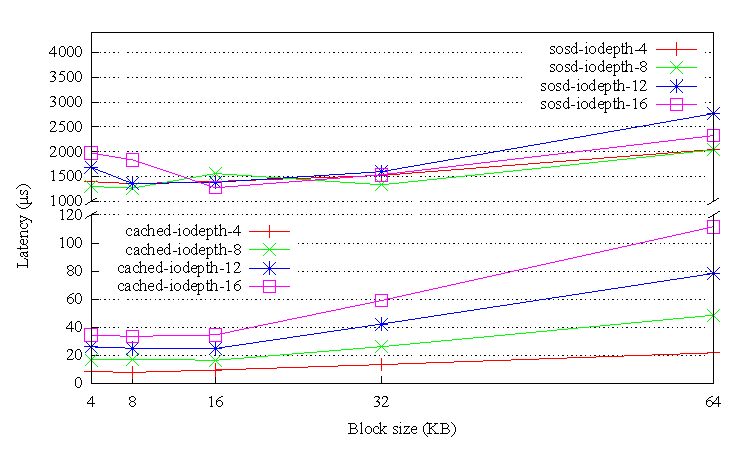
\includegraphics[width=\columnwidth]{images/lat-read-comp-lie.pdf}
			}
			Variables:
			\begin{itemize}
				\item block size [4KB - 64KB]
				\item parallel requests [4 - 16]
			\end{itemize}
		\end{column}
	\end{columns}

	\note[item]{Αντίστοιχα, για μικρά reads είμαστε 50x γρηγορότεροι ενώ 
		για μεγάλα έως 75x}
\end{frame}

\begin{frame}{Cached/sosd comparison - sustained behavior}
	\begin{columns}[t]
		\begin{column}{.5\textwidth}
			Write bandwidth
			\makebox[\textwidth]{
				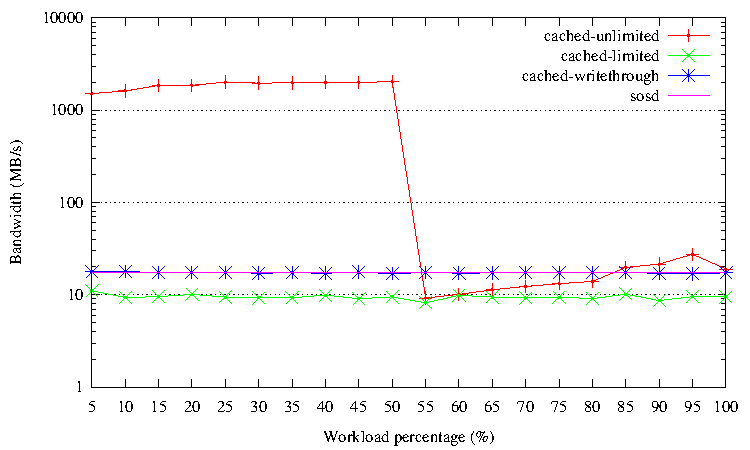
\includegraphics[width=\columnwidth]{images/bw-write-comp-truth.pdf}
			}
			Constants:
			\begin{itemize}
				\item cached has 4 threads
				\item workload twice the cache size
				\item block size is 4KB
				\item Parallel requests are 16
			\end{itemize}
		\end{column}
		\begin{column}{.5\textwidth}
			Write latency
			\makebox[\textwidth]{
				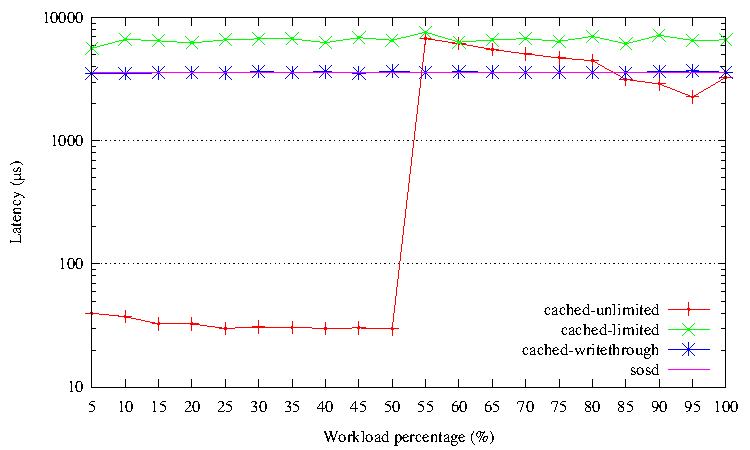
\includegraphics[width=\columnwidth]{images/lat-write-comp-truth.pdf}
			}
			Variables:
			\begin{itemize}
				\item cache write policy
				\item maximum cached objects
			\end{itemize}
		\end{column}
	\end{columns}

	\note[item]{unlimited: έχουμε περισσότερα buckets απ' ότι objects}
	\note[item]{Σημεία προσοχής: Writethrough όσο και το Rados ενώ στα 
		reads έχουμε παρατηρήσει καλύτερη ταχύτητα}
	\note[item]{Το performance πέφτει λόγω έλλειψης buckets, μεγαλώνει λόγω 
		coalesces}

\end{frame}

\begin{frame}{Cached internals - indexing}
	Latency of cold cache vs. warm cache
	\makebox[\textwidth]{
		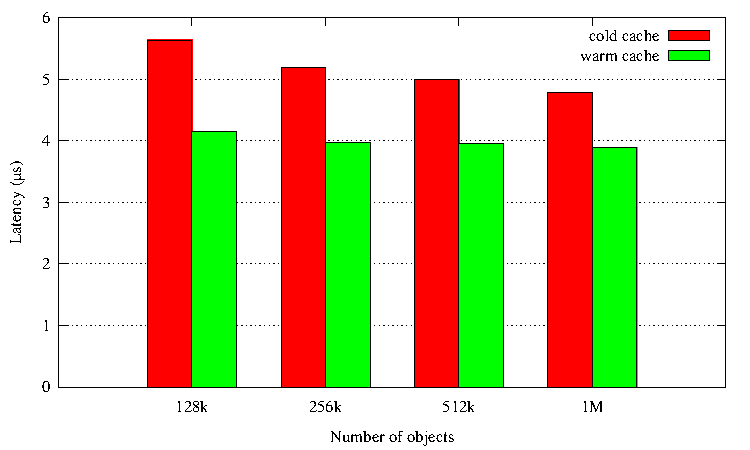
\includegraphics[width=0.45\textwidth]{images/cold1.pdf}
	}
	\begin{columns}[t]
		\begin{column}{.5\textwidth}
			Constants:
			\begin{itemize}
				\item workload less than the cache size
				\item block size is 4KB
				\item no threads or parallel requests 
			\end{itemize}
		\end{column}
		\begin{column}{.5\textwidth}
			Variables:
			\begin{itemize}
				\item number of objects [128k - 1M]
			\end{itemize}
		\end{column}
	\end{columns}
	\note[item]{Το σενάριο είναι το εξής. Εισάγουμε ένα αριθμό από objects.  
		Κάνουν lookup και insert. Μετά, τα κάνουμε lookup. Αυτό το κάνουμε για 
		128κ ... Μετράμε latency}
	\note[item]{Σταθερό indexing overhead. Αν πέσει ερώτηση πες 2Μ hash 
		table, το λειτουργικό δε δίνει αμέσως μνήμη}
\end{frame}

\begin{frame}{VM/Archipelago evaluation}
	\begin{columns}[t]
		\begin{column}{.5\textwidth}
			Write bandwidth
			\makebox[\textwidth]{
				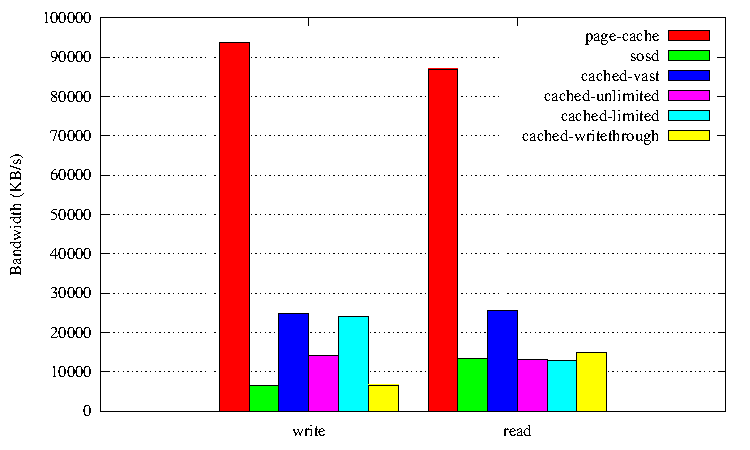
\includegraphics[width=\columnwidth]{images/bw-vm.pdf}
			}
			Constants:
			\begin{itemize}
				\item block size is 4KB
				\item parallel requests are 16
				\item cached has 4 threads
			\end{itemize}
		\end{column}
		\begin{column}{.5\textwidth}
			Write latency
			\makebox[\textwidth]{
				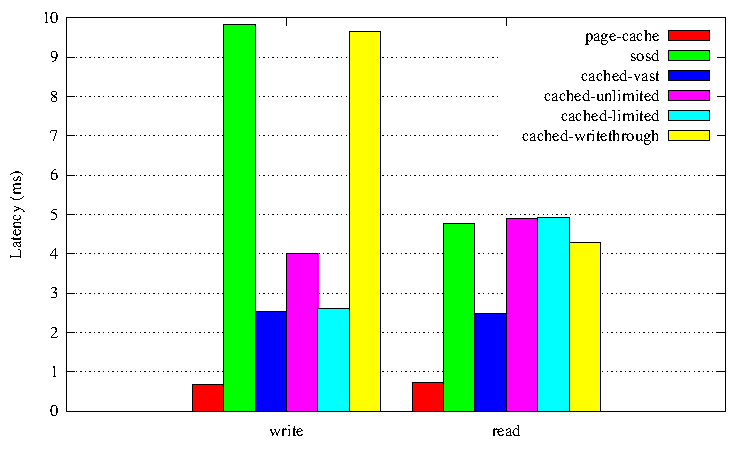
\includegraphics[width=\columnwidth]{images/lat-vm.pdf}
			}
			Variables:
			\begin{itemize}
				\item cache write policy
				\item maximum cached objects
			\end{itemize}
		\end{column}
	\end{columns}
	\note{Benchmark μέσα από το VM, με filesystem, elevators, κτλ. με το fio}
	\note{Σημεία προσοχής:
		\begin{itemize}
			\item page-cache: πολύ γρήγορη. Το 1ms latency λογικά 
				μπαίνει λόγω του paravirtualized storage, 
				filesystem, elevators
			\item sosd: είναι σίγουρα άσχημο αλλά σε αυτά τα test 
				έχει συν 7ms latency για τα writes και 3ms 
				latency για τα reads. Αυτό έιναι πολύ 
				μεγαλύτερο του 1ms του VM άρα κάτι παίζει με 
				Αρχιπέλαγο
			\item cached-vast: 4x γρηγορότερη από sosd αλλά έχει 
				3ms latency που δεν είχε πριν, δηλαδή το 
				archipelago βάζει 2ms
			\item cached-unlimited: 2.5x γρηγορότερο και ξεπέρασε 
				πάλι τον sosd στο τέλος
			\item cached-limited: 4x γρηγορότερο, λογικά τα flushes 
				είναι πολλα και μικρά και κρύβονται πίσω από το 
				latency του Archipelago
			\item writethrough δεν είδαμε κάποια διαφορά
		\end{itemize}
	}
\end{frame}





\chapter{The synapsed peer}\label{ch:synapsed}

On the previous sections, we have evaluated the design of cached and one of the 
conclusions that we have reached at is that it has heavy lock contention when 
more than one threads are used. The implications of this, however, are bigger, 
if we consider that Archipelago is running in the host machine, whose CPU's are 
already oversubscribed. This means that cached must compete for CPU time 
against the running VMs, essentially defeating the QoS purpose it serves.

On the other hand, on the RADOS nodes, the CPUs and RAM are not used to their 
full potential. If we could run cached or part of the Archipelago in these 
nodes, we would have the following benefits:

\begin{itemize}
	\item We would have access to a much larger amount of RAM
	\item We would make a big step forward in terms of creating a 
		distributed cache, since we would be able to replicate the data 
		to two or more cached peers that would ran in different nodes, 
		since these nodes are accessible from any host.
\end{itemize}

To this end, we have created a network peer called synapsed (from 
\textbf{synapse d}aemon) as a proof-of-concept, that should be able to accept 
read/write XSEG requests and send them through network to another Archipelago 
segment. We must note that this peer, given that it is proof-of-concept, has 
not been created with high-performance in mind but its main aim is to provide 
the functionality needed for our purposes.  As a consequence, we have not used 
tools such as ZeroMQ or libevent that would boost the performance of the 
implementation.

The structure of this chapter is the following. Section 
\ref{sec:design-synapsed} presents the design of the synapsed peer. Section 
\ref{sec:imp-synapsed} explains how we implemented synapsed as well as the 
challenges that we have faced. Finally, Section \ref{sec:plot-synapsed} 
provides the results of some preliminary benchmarks that we have conducted 
using synapsed.

\section{Design of synapsed}\label{sec:design-synapsed}

Given that currently Archipelago is not network-aware, peers from one segment 
cannot know the ports of peers of another segment. Moreover, they cannot send a 
request to the synapsed peer and simultaneously target a peer in another 
segment. So, we are faced with the problem of defining the limitations of 
synapsed.

We propose the following design: Each of these two segments must have at least 
one synapsed peer. So, when one synapsed accepts an XSEG request, it will 
translate it to a network request, send it to the synapsed peer of the other 
segment, who in turn will finally translate it back to an XSEG request.  
Moreover, each synapsed peer must be attached to a peer of its segment, which 
will serve as the request target when synapsed accepts a request.  

This means that synapsed does not actually connect two remote segments. More 
appropriately, it bridges two remote peers over network.

Another difficult task was to enable synapsed to listen from its port and its 
request queue simultaneously, using the request handling of Archipelago. We 
have tackled this problem in Section \ref{sec:poll-synapsed}.

Moreover, synapsed has been designed to send requests using the standard TCP 
protocol.  This means that it must handle the marshaling of buffers, 
send/receive errors as well as polling for new requests all by itself.

Finally, synapsed has been designed as a single-threaded peer.

\section{Implementation of synapsed}\label{sec:imp-synapsed}

In this section, we will explain how we implemented the main aspects of 
synapsed.

\subsection{Synapsed initialization}

Synapsed is a much simpler peer than cached and requires only the following 
arguments:

\begin{itemize}
	\item The network port where it will listen for requests.
	\item The remote address of the segment. \textbf{NOTE:} it can point to 
		the host address, which means that synapsed can also provide a 
		generic way to bridge two peers who reside in the same host but 
		in a different segment.
	\item The remote network port of the other synapsed peer.
	\item The XSEG port of the peer where synapsed will send the requests 
		that it accepts.
\end{itemize}

Once synapsed has the above arguments, it can create a socket, bind it and 
connect to its port. After that, it can listen for new connections and forward 
the requests that it receives to the synapsed of the other segment. That 
synapsed can in turn forward the request to the peer that it has been 
configured to target to.

\subsection{Request polling}\label{sec:poll-synapsed}

Synapsed typically uses the common peer polling and Archipelago IPC methods 
(see Section \ref{sec:arch-poll}) to check its XSEG ports for new requests.  
However, it simultaneously needs to listen for new requests on its socket. Yet, 
there is no way for a process to block on its socket \textbf{and} and 
synchronously wait for a queued signal.

The solution seems obvious; synapsed should instead block while polling for 
requests in its socket and, if a new request arrives at its XSEG port, its 
polling should be interrupted. This is a simple solution, but there is one
detail we must take into account; sleeping like so is unsafe because peers 
currently block the SIGIO signal in order to wake up synchronously.

Let's elaborate on that a bit: When a peer is initialized, it blocks the SIGIO 
signal. Using sigtimedwait, it can check fast and without races if a signal has 
been enqueued, and then it can sleep. This is not the case with \texttt{poll()} 
though, since if the peer sleeps with the SIGIO signal blocked, it will not 
wake up.  On the other hand, if we unblock the SIGIO signal, we have a new set 
of problems:

Consider the case where we receive a signal before we go to sleep. In order to 
be notified that a signal has been sent so as not to sleep, we would need to 
utilize a signal handler that would increment a global variable which would be 
checked right before we go to sleep. This approach is not only racy (what 
happens if SIGIO is received after this global variable is checked) but it is 
also very slow.

For this reason, we use the \texttt{ppoll()} alternative, which accepts a 
signal mask as an additional argument. \texttt{ppoll()} provides the guarantee 
that it will atomically: \begin{inparaenum}[i)]
\item replace the old signal mask of the process with the one provided,
\item check if there are pending signals and if so return,
\item block until a request has been received or a signal has been queued.
\end{inparaenum}

Solving the issue of waiting for XSEG requests while blocking on a socket is 
only part of the problem. We also have to solve its counterpart, which means we 
need to find a quick way to iterate the XSEG ports of synapsed for new 
requests, while listening for new requests on its socket.

We have countered this problem by checking alternately the XSEG port of 
synapsed, with the existing methods, and the network port of synapsed, by doing 
a poll with zero timeout, which returns immediately.

\subsection{Marshalling}

The XSEG request cannot be sent as is, since its data and target name are 
stored in two different buffers. Moreover, since these buffers can have 
variable length, the synapsed peer that reads from its socket needs a way to 
know when it has finished reading all the necessary data.

This is a common problem in computer science and its solution is to serialize 
(or "marshal") the object that must be transfered. The marshaling method we 
have chosen is the following:

\begin{enumerate}
	\item We send at the start of every transaction a fixed-length header, 
		whose size is known to all synapsed peers, and which has the 
		information about the length of the rest of the buffers.  The 
		header is presented on Listing \ref{lst:synapsed-header.h}

		\ccode{Synapsed header}{synapsed-header.h}

		The header is simply the necessary fields of the original 
		request that the remote synapsed peer needs to know. The most 
		important fields are \textbf{datalen} and \textbf{targetlen} 
		which indicate the length of the data and target buffers 
		respectively.
	\item Once the header has been sent and the remote peer has the 
		information that it needs, it allocates a new XSEG request from 
		its segment and fills it with the information provided by the 
		header, thereby creating to buffers with the appropriate 
		length.
	\item Finally, the remote synapsed peer reads the rest two buffers and 
		stores them in the XSEG request it has previously allocated.
\end{enumerate}

Marshaling however is usually not so simple. There are three caveats that one 
must take into account before attempting to serialize manually an object. They 
derive from the often overlooked fact that the host and the remote machine are 
not architecturally the same, which can lead to:

\begin{enumerate}
	\item \textbf{Different endianness}. This means that the two machines have 
		completely different byte order. This is commonly solved by converting 
		all of the data to network byte order (big endian) and then convert 
		them to the native endianess of the machine.
	\item \textbf{Different type representation}. Even if two architectures 
		have the same endianness, it is possible that they represent the same 
		types with different number of bytes. This is most common with 32-bit 
		and 64-bit architectures which, for example, use 4 bytes and 8 bytes 
		respectively to represent an int.
	\item \textbf{Padding}. Due to data alignment issues, the compiler may 
		need to pad the fields of a struct. The padding is depended on 
		the processor that is used to compile the program. A common 
		solution to sidestep padding issues from different processors 
		is to "pack" the structure, i.e.  to enforce that the structure 
		will have no padding.
\end{enumerate}

For synapsed, the first two caveats do not affect us, since the machines that 
are used are both 64-bit, little endian machines. The third caveat may also not 
affect us, but just to make sure, we have packed our header structure using the 
gcc pragma directive:

\ccode{GCC pragma pack directive}{synapsed-pack.h}

\subsection{Send/Receive}

As we have mentioned in the previous chapter, in order to send the data from 
one synapsed peer to the other, we must marshal them first and then unmarshal 
them. This commonly requires to merge all buffers into one and send that 
buffer.  

In synapsed however, we have chosen a different approach; we have employed the 
\texttt{readv()}/\texttt{writev()} functions, that allow us to do 
scatter/gather I/O.

This means that when we sent a request, we create an iovec vector that points 
to the data that we want to sent and their sizes (gather). Respectively, when 
we receive a request, we check its type and allocate the necessary XSEG buffers 
where the data can be copied (scatter).

\section{Evaluation of synapsed}\label{sec:plot-synapsed}

Currently, synapsed is in a functional but nascent state, meaning that 
important features such as mirroring of requests have not been implemented yet.  
Were these features implemented, they could also be evaluated and we would be 
able to quantify their performance cost.

This means that right now, synapsed's main purpose is to enable cached and 
other Archipelago peers to work in a remote environment with more resources, 
without encumbering the host machine. This kind of flexibility cannot be 
evaluated of course, but it should be considered an important feat, since it 
opens numerous possibilities for a previously network-unaware Archipelago.

There is however an interesting way we can evaluate synapsed. More 
specifically, we can benchmark its performance for each of the Archipelago 
configurations that are tested in Section \ref{sec:vm-plot}, minus the page 
cache test of course. 

The setup for our benchmarks is identical to the setup that is used in Chapter 
\ref{ch:cached-evaluation}. The only addition is that synapsed is in a 
different host, with similar specifications as our test-bed (see Section 
\ref{sec:test-bed}).  Additionally, the two hosts are connected with a 1Gbit 
Ethernet cable. Note that neither this connection type nor synapsed are tuned 
for high performance.  This is important in order to properly evaluate the 
following results.

We proceed with the performance results of our benchmarks. The bandwidth 
results are presented in Figure \ref{fig:bw-write-synapsed.pdf} and the latency 
results in Figure \ref{fig:lat-write-synapsed.pdf}.

\diagram{Bandwidth performance for writes through 
	synapsed}{bw-write-synapsed.pdf}
\diagram{Latency performance for writes through 
	synapsed}{lat-write-synapsed.pdf}

For the first round of comparisons, will be invoke the results of Section 
\ref{sec:sustained-plot} and more specifically Figures 
\ref{fig:bw-write-comp-truth.pdf} and \ref{fig:lat-write-comp-truth.pdf}.

The first impression that one gathers by comparing these results is that they 
seem very similar but clipped. This is expected since the theoretical maximum 
bandwidth of a 1Gbit ethernet cable is 128MB/s. The fastest that we seem to 
reach is 110MB/s, which is very close, if we consider that on the same cable 
both peers send data simultaneously. 

Most importantly however, besides the clipping in fast scenarios, there is 
practically little or no other effect on the rest of the scenarios, as they 
have approximately the same speed, with synapsed being only a little slower.

Moreover, we can see that cached-unlimited is performing similarly in both 
benchmarks and once again manages to outperform sosd, albeit being noticeably 
slower in the synapsed benchmark.

From the above comparisons we can observe that the network can be a bottleneck 
for an I/O intensive application, especially when it can achieve higher 
bandwidth than what the network can sustain.

We conclude this section with a comparison of our results with the results of 
Figures \ref{fig:bw-vm.pdf} and \ref{fig:lat-vm.pdf}. As we can see in these 
results, the latency that is introduced by the VM operations, hypervisor and 
Archipelago is currently far greater than the < 1ms latency of the 1Gbit 
connection. Moreover, if the connection between the two servers were 10G, the 
latency that is imposed by the network would be negligible.

What we try to infer with the above observation is that in the current 
situation, the network latency of synapsed is a small price to pay if we can 
manage to run cached or even Archipelago in a remote environment with more RAM.

\chapter{Conclusion}\label{ch:future}

\section{Concluding remarks}

This thesis is a record of over a year long process that has ultimately lead to 
the creation of two Archipelago peers, cached and synapsed. It documents the 
evaluation of third-party solutions, the reasoning behind our choice to create 
a custom cache mechanism, as well as the design decisions and technical issues 
that we have encountered.

Looking back at what we have created, we can safely state that this thesis has 
successfully covered two basic needs of Archipelago, caching and networking.  
The extend at which these needs have been satisfied can be considered as more 
than adequate, since cached has been successfully tested under an actual VM, 
while synapsed has managed to bridge two peers over network with minimum 
latency.

Most importantly however, cached provides a concrete solution to the task that 
was described in the very first chapter of this thesis; substantially improve 
the current performance of Archipelago.  To be more specific, the results of 
synthetic benchmarks show that cached can improve up to 200x the current 
performance.  Moreover, when tested with an actual VM, the performance speedup 
was able to reach 400\%, even for small cache sizes.

Finally, the future looks very bright for our caching mechanism. The impending 
integration of cached in the demo environment\footnote{demo.synnefo.org}
of Synnefo, will help it gain the necessary exposure that will provide us with 
the needed feedback for more improvements and the test-bed for new ideas.

\section{Future work}

The future work for cached is happening as of writing this very chapter. We are 
currently working to add the following:

\begin{itemize}
	\item Full CoW support.
	\item Support for different namespaces (mappings, volumes, objects) so 
		that cached can be used as a generic caching peer for all 
		Archipelago needs.
	\item Support for different policies and limits per volume.
\end{itemize}

Moreover, the long term goal for cached is to be able to be used with synapsed 
effectively, in order to create a fast distributed and replicated cache.



\backmatter
\cleardoublepage % start at the next odd page
\phantomsection % correct hyperlinking
\bibliography{references}
\bibliographystyle{plain}
% \newcommand{\gloss}[2]{#1 \> \en{#2}\\ }

\chapter{����������� ����� ����}

\begin{tabbing}
%ta 'a' rythmizoun to platos ton dyo stilon
  aaaaaaaaaaaaaaaaaaaaaaaaaaaaaaaaaaa \= aaaa\kill
  \Large\textbf{���������} \> \Large\textbf{�������� ����} \\
  \gloss{�������}{sibling}
  \gloss{��������������}{idempotency}
  %\gloss{������������}{identifier}
  \gloss{�������� �����������}{information retrieval}
  \gloss{������������������}{commutativity}
  \gloss{��������}{descedant}
  \gloss{����������}{absorption}
  \gloss{���� ���������}{database}
  \gloss{��������}{attribute}
  \gloss{������������}{interface}
  \gloss{�������}{difference}
  \gloss{��������� ���������}{portal catalog}
  \gloss{�������� ����}{lattice}
  \gloss{������� �����������}{structural queries}
  \gloss{������� �������}{structural relationships}
  \gloss{������ �����}{schema}
  \gloss{����������}{validity}
  \gloss{�����}{union}
\end{tabbing}

% \chapter{Appendix}
% \printindex

\end{document}
